%% (Master) Thesis template
% Template version used: v1.4
%
% Largely adapted from Adrian Nievergelt's template for the ADPS
% (lecture notes) project.


%% We use the memoir class because it offers a many easy to use features.
\documentclass[11pt,a4paper,titlepage]{memoir}

%% Packages
%% ========

%% LaTeX Font encoding -- DO NOT CHANGE
\usepackage[OT1]{fontenc}

%% Babel provides support for languages.  'english' uses British
%% English hyphenation and text snippets like "Figure" and
%% "Theorem". Use the option 'ngerman' if your document is in German.
%% Use 'american' for American English.  Note that if you change this,
%% the next LaTeX run may show spurious errors.  Simply run it again.
%% If they persist, remove the .aux file and try again.
\usepackage[english]{babel}

%% Input encoding 'utf8'. In some cases you might need 'utf8x' for
%% extra symbols. Not all editors, especially on Windows, are UTF-8
%% capable, so you may want to use 'latin1' instead.
\usepackage[utf8]{inputenc}

%% This changes default fonts for both text and math mode to use Herman Zapfs
%% excellent Palatino font.  Do not change this.
\usepackage[sc]{mathpazo}

%% The AMS-LaTeX extensions for mathematical typesetting.  Do not
%% remove.
\usepackage{amsmath,amssymb,amsfonts,mathrsfs,stmaryrd}

%% NTheorem is a reimplementation of the AMS Theorem package. This
%% will allow us to typeset theorems like examples, proofs and
%% similar.  Do not remove.
%% NOTE: Must be loaded AFTER amsmath, or the \qed placement will
%% break
\usepackage[amsmath,thmmarks]{ntheorem}

%% LaTeX' own graphics handling
\usepackage{graphicx}

%% This allows you to add .pdf files. It is used to add the
%% declaration of originality.
\usepackage{pdfpages}

%% This package allows you to easily typeset grammars for programming languages
\usepackage{plstx}

%% This package allows you to format proof trees
\usepackage{bussproofs}

%% For sticking out todo notes and random notes for me
\newcommand{\TODO}[1]{\textcolor{red!60!black}{\textbf{TODO:}~#1}}
\newcommand{\note}[1]{\textcolor{blue!60!red}{~#1}}

%% Some more packages that you may want to use.  Have a look at the
%% file, and consult the package docs for each.
%% See the TeXed file for more explanations

%% [OPT] Multi-rowed cells in tabulars
%\usepackage{multirow}

%% [REC] Intelligent cross reference package. This allows for nice
%% combined references that include the reference and a hint to where
%% to look for it.
\usepackage{varioref}

%% [OPT] Easily changeable quotes with \enquote{Text}
%\usepackage[german=swiss]{csquotes}

%% [REC] Format dates and time depending on locale
\usepackage{datetime}

%% [OPT] Provides a \cancel{} command to stroke through mathematics.
%\usepackage{cancel}

%% [NEED] This allows for additional typesetting tools in mathmode.
%% See its excellent documentation.
\usepackage{mathtools}

%% [ADV] Conditional commands
%\usepackage{ifthen}

%% [OPT] Manual large braces or other delimiters.
%\usepackage{bigdelim, bigstrut}

%% [REC] Alternate vector arrows. Use the command \vv{} to get scaled
%% vector arrows.
\usepackage[h]{esvect}

%% [NEED] Some extensions to tabulars and array environments.
\usepackage{array}

%% [OPT] Postscript support via pstricks graphics package. Very
%% diverse applications.
%\usepackage{pstricks,pst-all}

%% [?] This seems to allow us to define some additional counters.
%\usepackage{etex}

%% [ADV] XY-Pic to typeset some matrix-style graphics
%\usepackage[all]{xy}

%% [OPT] This is needed to generate an index at the end of the
%% document.
%\usepackage{makeidx}

%% [OPT] Fancy package for source code listings.  The template text
%% needs it for some LaTeX snippets; remove/adapt the \lstset when you
%% remove the template content.
\usepackage{listings}

%% Package for algorithms
\usepackage{algorithm2e}

%% [REC] Fancy character protrusion.  Must be loaded after all fonts.
\usepackage[activate]{pdfcprot}

%% [REC] Nicer tables.  Read the excellent documentation.
\usepackage{booktabs}

%% Convert .eps to .pdf for pfdlatex
\usepackage{epstopdf}


%% Our layout configuration.  DO NOT CHANGE.
%% Memoir layout setup

%% NOTE: You are strongly advised not to change any of them unless you
%% know what you are doing.  These settings strongly interact in the
%% final look of the document.

% Dependencies
\usepackage{ETHlogo}

% Turn extra space before chapter headings off.
\setlength{\beforechapskip}{0pt}

\nonzeroparskip
\parindent=0pt
\defaultlists

% Chapter style redefinition
\makeatletter

\if@twoside
  \pagestyle{Ruled}
  \copypagestyle{chapter}{Ruled}
\else
  \pagestyle{ruled}
  \copypagestyle{chapter}{ruled}
\fi
\makeoddhead{chapter}{}{}{}
\makeevenhead{chapter}{}{}{}
\makeheadrule{chapter}{\textwidth}{0pt}
\copypagestyle{abstract}{empty}

\makechapterstyle{bianchimod}{%
  \chapterstyle{default}
  \renewcommand*{\chapnamefont}{\normalfont\Large\sffamily}
  \renewcommand*{\chapnumfont}{\normalfont\Large\sffamily}
  \renewcommand*{\printchaptername}{%
    \chapnamefont\centering\@chapapp}
  \renewcommand*{\printchapternum}{\chapnumfont {\thechapter}}
  \renewcommand*{\chaptitlefont}{\normalfont\huge\sffamily}
  \renewcommand*{\printchaptertitle}[1]{%
    \hrule\vskip\onelineskip \centering \chaptitlefont\textbf{\vphantom{gyM}##1}\par}
  \renewcommand*{\afterchaptertitle}{\vskip\onelineskip \hrule\vskip
    \afterchapskip}
  \renewcommand*{\printchapternonum}{%
    \vphantom{\chapnumfont {9}}\afterchapternum}}

% Use the newly defined style
\chapterstyle{bianchimod}

\setsecheadstyle{\Large\bfseries\sffamily}
\setsubsecheadstyle{\large\bfseries\sffamily}
\setsubsubsecheadstyle{\bfseries\sffamily}
\setparaheadstyle{\normalsize\bfseries\sffamily}
\setsubparaheadstyle{\normalsize\itshape\sffamily}
\setsubparaindent{0pt}

% Set captions to a more separated style for clearness
\captionnamefont{\sffamily\bfseries\footnotesize}
\captiontitlefont{\sffamily\footnotesize}
\setlength{\intextsep}{16pt}
\setlength{\belowcaptionskip}{1pt}

% Set section and TOC numbering depth to subsection
\setsecnumdepth{subsection}
\settocdepth{subsection}

%% Titlepage adjustments
\pretitle{\vspace{0pt plus 0.7fill}\begin{center}\HUGE\sffamily\bfseries}
\posttitle{\end{center}\par}
\preauthor{\par\begin{center}\let\and\\\Large\sffamily}
\postauthor{\end{center}}
\predate{\par\begin{center}\Large\sffamily}
\postdate{\end{center}}

\def\@advisors{}
\newcommand{\advisors}[1]{\def\@advisors{#1}}
\def\@department{}
\newcommand{\department}[1]{\def\@department{#1}}
\def\@thesistype{}
\newcommand{\thesistype}[1]{\def\@thesistype{#1}}

\renewcommand{\maketitlehooka}{\noindent\ETHlogo[2in]}

\renewcommand{\maketitlehookb}{\vspace{1in}%
  \par\begin{center}\Large\sffamily\@thesistype\end{center}}

\renewcommand{\maketitlehookd}{%
  \vfill\par
  \begin{flushright}
    \sffamily
    \@advisors\par
    \@department, ETH Z\"urich
  \end{flushright}
}

\checkandfixthelayout

\setlength{\droptitle}{-48pt}

\makeatother

% This defines how theorems should look. Best leave as is.
\theoremstyle{plain}
\setlength\theorempostskipamount{0pt}

%% This defines how your lstlistings look like
\lstdefinestyle{plain}{%
    language=ML,
    basicstyle={\normalfont\ttfamily},
	tabsize=2,
}

\lstdefinestyle{algorithm}{%
    mathescape,
    basicstyle={\normalfont\small},
	tabsize=2,
	keywordstyle=\textbf,
	otherkeywords={while,if,else,for,end,Input,Output},
	literate={:=}{{$\gets$}}1 {=<}{{$\leq$}}1 {>=}{{$\geq$}}1 {<>}{{$\neq$}}1{->}{$\rightarrow$}1,
}

%%% Local Variables:
%%% mode: latex
%%% TeX-master: "thesis"
%%% End:


%% Theorem environments.  You will have to adapt this for a German
%% thesis.
%% Theorem-like environments

%% This can be changed according to language. You can comment out the ones you
%% don't need.

\numberwithin{equation}{chapter}

%% German theorems
%\newtheorem{satz}{Satz}[chapter]
%\newtheorem{beispiel}[satz]{Beispiel}
%\newtheorem{bemerkung}[satz]{Bemerkung}
%\newtheorem{korrolar}[satz]{Korrolar}
%\newtheorem{definition}[satz]{Definition}
%\newtheorem{lemma}[satz]{Lemma}
%\newtheorem{proposition}[satz]{Proposition}

%% English variants
\newtheorem{theorem}{Theorem}[chapter]
\newtheorem{example}[theorem]{Example}
\newtheorem{remark}[theorem]{Remark}
\newtheorem{corollary}[theorem]{Corollary}
\newtheorem{definition}[theorem]{Definition}
\newtheorem{lemma}[theorem]{Lemma}
\newtheorem{proposition}[theorem]{Proposition}

%% Proof environment with a small square as a "qed" symbol
\theoremstyle{nonumberplain}
\theorembodyfont{\normalfont}
\theoremsymbol{\ensuremath{\square}}
\newtheorem{proof}{Proof}
%\newtheorem{beweis}{Beweis}


%% Helpful macros.
%% Custom commands
%% ===============

%% Special characters for number sets, e.g. real or complex numbers.
\newcommand{\C}{\mathbb{C}}
\newcommand{\K}{\mathbb{K}}
\newcommand{\N}{\mathbb{N}}
\newcommand{\Q}{\mathbb{Q}}
\newcommand{\R}{\mathbb{R}}
\newcommand{\Z}{\mathbb{Z}}
\newcommand{\X}{\mathbb{X}}

%% Fixed/scaling delimiter examples (see mathtools documentation)
\DeclarePairedDelimiter\abs{\lvert}{\rvert}
\DeclarePairedDelimiter\norm{\lVert}{\rVert}

%% Use the alternative epsilon per default and define the old one as \oldepsilon
\let\oldepsilon\epsilon
\renewcommand{\epsilon}{\ensuremath\varepsilon}

%% Also set the alternate phi as default.
\let\oldphi\phi
\renewcommand{\phi}{\ensuremath{\varphi}}


%% Make document internal hyperlinks wherever possible. (TOC, references)
%% This MUST be loaded after varioref, which is loaded in 'extrapackages'
%% above.  We just load it last to be safe.
\usepackage[linkcolor=black,colorlinks=true,citecolor=black,filecolor=black]{hyperref}


%% Document information
%% ====================

\title{Inductive Synthesis from Higher-Order Functions}
\author{Alexandra Maximova}
\thesistype{Master Thesis}
\advisors{Advisors: Prof.\ Dr.\ Martin Vechev, Dimitar Dimitrov}
\department{Department of Computer Science}
\date{August 15, 2016}

\begin{document}

\frontmatter

%% Title page is autogenerated from document information above.  DO
%% NOT CHANGE.
\begin{titlingpage}
  \calccentering{\unitlength}
  \begin{adjustwidth*}{\unitlength-24pt}{-\unitlength-24pt}
    \maketitle
  \end{adjustwidth*}
\end{titlingpage}

%% The abstract of your thesis.  Edit the file as needed.
\begin{abstract}

We investigate the benefits of providing a relatively large library of components to a program synthesiser. Library components encode well-known computational patterns that human programmers reuse in their programs. We target the synthesis of functional straight-line programs from input-output examples. We implement a basic synthesis algorithm based on best-first enumeration combined with type-based pruning. We use heuristics to guide the search and black lists to prune the search space. We have evaluated our prototype implementation on simple algorithmic problems over a library of $37$ components. Results indicate that our basic algorithm performs not considerably worse that much more sophisticated state-of-the-art algorithms.

\end{abstract}


%% TOC with the proper setup, do not change.
\cleartorecto
\tableofcontents
\mainmatter

%% Your real content!
% Some commands used in this file
\newcommand{\package}{\emph}

\chapter{Introduction}\label{ch:introduction}

Let us move on to the contributions. We implemented in OCaml a prototype\footnote{\TODO{Link to the code?}} of the synthesis procedure we define in Chapter~\ref{ch:definitions}. The main contribution of this thesis is the extensive evaluation of our synthesis tool and the exploration of the search space. The experiments and the findings are presented in Chapter~\ref{ch:evaluation}.

The rest of the thesis is structured as follows. In Chapter~\ref{ch:definitions} the top-down synthesis procedure is introduced and formally defined. Chapter~\ref{ch:implementation} describes how to turn this synthesis procedure into a synthesis tool written in OCaml. In Chapter~\ref{ch:relatedwork} we shortly review four closely related synthesis tools: \textsc{Synquid} \cite{SynquidPaper}, $\lambda^2$ \cite{LambdaSquarePaper}, \textsc{Escher} \cite{EscherPaper} and \textsc{Myth} \cite{Mythpaper}. In Chapter~\ref{ch:evaluation} we present the results of the empiric evaluation. Finally, Chapter~\ref{ch:conclusions} draws the conclusions and outlines the possibilities for future work.

\TODO{Write this chapter\\}

\section{What is program synthesis?}

\section{Background}

\section{Problem}
We restrict ourselves to purely functional programs without pattern matching, without recursion, without conditionals, just application of library components and input variables. Handle many components. Reuse common knowledge. Computational patterns encoded as components.






----------------------------------
Plain and simple definition. Program synthesis is the automatic generation of programs. That's what programmers usually do: translate a, mostly oral and ambiguous, specification into a program that satisfies the specification. Wouldn't it be great, if computers once could do the same? (not really, but we leave the ethic and economic reasons out of scope. On the other hand, it would be just like compilers).

What's the problem? Why don't you know what to write in this chapter? It shouldn't be that difficult. You need
\begin{itemize}
\item general introduction/motivation. Don't forget to say what is program synthesis. "What is program synthesis"
\item background section "The problem is too general. Other restricted it in this and this way, tried this and this approach. Logical specification and deduction, input-output examples and induction, restrict to a particular domain like sketch and the bit-manipulating things or igor for number series. flashfill in excel gibt es auch noch. For functional programs we have this and this approaches and this and this restrictions"
\item intuitive description of the problem statement and a motivation why something that restricted should be interesting (encode computational patterns as components, thin interfaces, SKI as components). Bring the replicate example. Type-driven, example-based, from components. Should be stated clearly. "How I restrict the search space and what specification do I choose. Replicate example. Motivate why it could be useful and why this is not too restricted." Don't forget the main hypothesis, that higher-order components help.
\item list of contributions (what are my contributions? The algorithm is standard, the implementation is not really a contribution. Evaluation? Should I stress that this is empirical work?) "Move on to the contributions. Implementation and extensive empirical evaluation".
\item structure of the thesis (formal definition of the synthesis procedure, implementation, four closely related tools, evaluation). Well, you know how to write those sections :)
\end{itemize} 


Unlike our synthesis procedure, all of these tools are capable of synthesising recursive programs. This is not really a limitation, since common recursive patterns can be encoded as components. For example, the program \lstinline!p n = foldNatNat f init n! can be translated into the recursive program
\TODO{Make sure it is \lstinline!f (n-1) (p (n-1))! and not \lstinline!f n (p (n-1))!, correct if needed\\}
\begin{lstlisting}[style=plain]
p n = match n with
  | 0 -> init
  | n -> f (n-1) (p (n-1))
\end{lstlisting}  

for motivation you could write something about the extremely restricted list library in ocaml :)\\
Consider you are writing code in a functional programming language with a smaller choice of library functions than you are used to. For example (true story), if you are using OCaml and you are surprised that \lstinline?replicate? is missing even in the more complete core library \note{cite jane street core}, you could spend a couple of minutes writing your recursive version of \lstinline?replicate?. Or you can synthesize it with \textsc{Tamandu} in less than one second from other components. \TODO{rewrite without 'you' and maybe don't mention ocaml, core and all that thing?}.

input-output examples are an intuitive and simple way to specify programs and make synthesis more accessible to users with a lower level of expertise.


Problem definition: have many components, put them together into a program, no lambdas, no if-then-else, no recursion
  

  
  
Contributions: Evaluation, exploring the baseline algorithm, exploring the search space

\lstset{style=plain}

\chapter{Related Work} \label{ch:relatedwork}

In this chapter we look at four state-of-the-art tools closely related to our work. They all synthesise functional programs, are based on inductive enumeration and use type information to restrict the search space. Since simple types are too ambiguous to specify a program, the tools we present either choose to complement type information with input-output examples or resort to more complex and more expressive types that can actually act as a specification, as for example the \emph{refinement types} from \cite{SynquidPaper}.

\section{\mdseries\textsc{Synquid}}

In \cite{SynquidPaper} \textsc{Synquid} is proposed. The code can be found online\footnote{https://bitbucket.org/nadiapolikarpova/synquid} and there is the possibility to try it in the browser.
This tool uses \emph{refinement types} (types decorated with logical predicates) to prune the search space and to specify programs. SMT-solvers are used to satisfy the logical predicates appearing in the types.\\
Refinement types were already successfully used for verification. In particular, the tool builds upon the liquid types framework \cite{LiquidTypes}. However, it proposes a new procedure for type inference (called modular refinement type reconstruction), which thank to its modularity scales better than other existing inference procedures for refinement types. Programs can therefore be type checked even before they are put together.

This tool targets a language that includes lambda expressions, pattern matching, structural recursion, conditionals and fixpoint.
The user can define custom functions and inductive datatypes that can be passed to the synthesiser as components.

A program is specified by providing a type signature. For example, the synthesis goal \lstinline!replicate! can be specified as follows.
\begin{lstlisting}[style=plain]
n : Nat -> x : $\alpha$ -> {List $\alpha$ | len $\nu$ = n}
\end{lstlisting}
This is a dependent function type that denotes functions that, given a natural number $n$ and an $x$ of type $\alpha$, return a list of $\alpha$ of length $n$. Here $\nu$ is a special logical value variable that in this case denotes the runtime return value of the functions and \lstinline!len! is a measure function defined over lists.

This form of specification can be a disadvantage, since it is not that accessible to users with a lower level of expertise as input-output examples. It is not always easy to see which measure function for a custom datatype will lead to the most simple and intuitive specification.
On the other hand, refinement types allow to express programs that manipulate data structures with non-trivial universal and inductive invariants in a concise way. This allows to synthesise programs on sorted lists, unique lists, binary search trees, heaps and red-black trees.

This tool synthesises simple programs over lists and integers in under \SI{0.4}{s}. It can also handle more complex benchmarks that are out of the scope of this thesis, such as different sorting algorithms and manipulations of data structures with complex invariants. Various sorting algorithms over lists and trees are synthesised in under \SI{5}{s}. The synthesis of the most complex benchmark, the balancing of a red-black tree, takes up to \SI{20}{s}.

In contrast to our tool, the number of components provided to the synthesiser for evaluation is small.

\section{$\lambda^2$}
The tool proposed in \cite{LambdaSquarePaper} is called $\lambda^2$ and generates its output in $\lambda$-calculus with algebraic types and recursion. The target language also includes $7$ higher-order combinators such as \lstinline!map!, \lstinline!fold! and \lstinline!filter! and a flexible set of primitive operators and constants.

The user specifies the desired program providing only input-output examples. No particular knowledge is required from the user, as was demonstrated using randomly generated input-output examples. The goal type is inferred from the examples.

The synthesis algorithm is a combination of inductive generalisation, a limited form of deduction and enumerative search.
First, it generates \emph{hypotheses} in a type-aware manner, that is programs with free variables such as \lstinline!$\lambda$x. map ?f x! where \lstinline!?f! is a placeholder for an unknown program to be synthesised.
Then deduction in form of hand-coded rules about the higher-order combinators is used either to refute a hypothesis or infer new input-output examples to guide the synthesis of missing functions. For example, the hypothesis \lstinline!$\lambda$x. map ?f x! will be refuted if the length of the input list does not match the length of the output length.
Enumerative search is used to enumerate candidate programs to fill in the missing parts of hypotheses. Hypotheses and candidate programs are organised in a priority queue and, at each point of the search, the least-cost candidate is picked.

This tool is able to synthesize programs manipulating recursive data structures like lists, trees and nested data structures such as lists of lists and trees of lists.
It synthesises all benchmark programs in under 7~minutes. Half of the benchmarks is synthesised in under \SI{0.43}{s}. However, the synthesis of \lstinline!droplast!, the program that drops the last element of a list, takes up to \SI{320}{s}. The program that removes duplicates from a list, the program that drops the smallest elements of each list of a list of lists and the program that inserts a tree under each leaf of another tree take more than \SI{100}{s} to synthesise.

Unlike \textsc{Synquid} and our work, this tool can only use the $7$ hard-coded higher-order combinators. The extension of the set of higher-order combinators with own functions is not easily supported.


\section{\mdseries\textsc{Escher}}

In \cite{EscherPaper} \textsc{Escher} is presented. This tool targets a simple untyped purely functional language consisting of constants, input variables, conditionals and library components applied to all of their arguments, including a special component \lstinline!self! referring to the program being synthesised. This last component is used to synthesise recursive programs.

The user specifies the desired program as a \emph{closed} set of input-output examples. That is, for each input-output example, all examples needed to evaluate every recursive call must be present. For example, if we want to specify \lstinline!replicate! as
\begin{lstlisting}[style=plain]
replicate 2 'a' = ['a','a'],
\end{lstlisting}
we also need to provide the input-output examples for the possible recursive calls, that is
\begin{lstlisting}[style=plain]
replicate 1 'a' = ['a']
replicate 0 'a' = [].
\end{lstlisting}
This is necessary because recursive programs are evaluated using the input-output examples as an oracle. However, it is not always easy for an inexperienced user to provide such a set.

The search is goal-directed. Programs are associated with value vectors, that is the vector of the outputs of the program on the inputs from the input-output examples. Programs sharing the same value vectors are considered equivalent, that is the search space is pruned based on observational equivalence.
The algorithm alternates between two phases: forward search and conditional inference. During forward search programs are inductively enumerated by adding new components to already synthesised programs. During conditional inference a novel data structure, the \emph{goal graph}, is used to detect when two synthesised programs can be joined by a conditional statement. The alternation between the two phases is guided by a heuristic.

This tool is able to synthesise recursive programs, including tail recursive, mutually recursive and divide-and-conquer. It synthesises all benchmarks in under \SI{11}{s} and all but three benchmarks in under \SI{1}{s}. The benchmarks include programs on integers such as \lstinline!fibonacci! and \lstinline!isEven!, programs on lists such as \lstinline!compress! and \lstinline!insert! and programs on trees such as \lstinline!nodes-at-level! and \lstinline!count-leaves!.

Like our work, this tool can handle a flexible set of components. For example, a set of $23$ components was used to evaluate all benchmarks. However, there was no higher-order component among them.

\section{\mdseries\textsc{Myth}}
\TODO{Write this section\\}
Myth (Osera). Like mine, requires type and I/O-examples. Refinement tree.
\begin{enumerate}
\item What is the specification?
A type signature, the components and a list of input-output examples.
\item What is the target language?
pattern matching, recursion, higher-order functions in typed programming languages. Can synthesise higher-order functions, programs using higher-order functions and work with large algebraic datatypes.
ML-like language with algebraic data types, match, top-level function definitions and explicitly recursive functions.
\item What can they do well and fast? How fast?
Recursive programs with pattern matching. It's very fast, many programs are synthesised in around 0.1~s. It can also generate larger programs (75 AST nodes) in reasonable time (3~s for calculating the set of free variables in an untyped lambda-calculus).
\item What is the difficulty? What can they not generate (or take a long time)? How much time do they need?
To generate recursive functions, they also need a closed set of examples, so that a recursive call to the function being synthesised can be answered by an input-output example. They also require relatively many examples. They use a relatively large context, but they do not say how big it is.
Lacks support richer types like products and polymorphic types.
\item What do they do?
The tool in \cite{MythPaper} is called \textsc{Myth} and uses not only type information but also input-output examples to restrict the search space. The special data structure used to hold this information is the \emph{refinement tree}. This system can synthesize higher-order functions, programs that use higher order functions and work with large algebraic data types.\\
There is an ML-like type system that incorporates input-output examples. Two pieces: a \emph{refinement tree} and an enumerative search.\\
Two major operations: refine the goal type and the examples (push them down in the refinement tree) and guess a term of the right type that matches the examples (for one of the nodes of the refinement tree).\\
\end{enumerate}





%Leon (can bring it, it's deductive, so it's different than the others. It also targets functional programs. No, I have nothing to compare. The benchmark is too different.) \cite{LeonPaper}
%\begin{enumerate}
%\item What is the specification?
%Input-output relations (including examples), pre- and postconditions.
%\item What is the target language?
%Several recursion schemas (only terminating programs), components, pattern matching
%\item What can they do well and fast? How fast?
%The good thing is that they generate verified software. And it's interactive, the user can control the structure if he wants to.
%\item What is the difficulty? What can they not generate (or take a long time)? How much time?
%
%\item What do they do?
%Deductive synthesis, counterexample-guided.
%That's from the verification side: the point is to deliver \emph{verified} software that satisfies some specifications such as assertions, pre-conditions and post-conditions.
%\end{enumerate}


%%% Local Variables:
%%% mode: latex
%%% TeX-master: "thesis"
%%% End:

\lstset{style=plain}

\chapter{A type-driven synthesis procedure} \label{ch:definitions}

In this chapter we will formally define our type-directed top-down synthesis procedure. We will start with an intuitive description thereof based on an example and move on to the formal definitions, starting with the target programming language and the search space. Finally, we will present some enhancements.

\section{The 'replicate' example}

Recall the example from Chapter~\ref{ch:introduction} where we wanted to synthesise the program corresponding to \lstinline?replicate.? As our synthesis procedure is type-driven and example-based, the user specifies a program by providing its type along with a few I/O-examples.\\
Let us specify \lstinline?replicate? as follows.
\begin{lstlisting}[style=plain]
replicate :: $\forall$X. Int -> X -> List X
replicate 3 1 = [1,1,1]
replicate 2 [] = [[],[]]
\end{lstlisting}

We also need a library of components from which we are going to compose our program. Let us assume that our library contains the standard list combinators \lstinline?map? and \lstinline?foldr?, \lstinline?enumTo?, that is the function that returns a list from $1$ up to its argument, and \lstinline?const?, that is the function that always returns its first argument. Moreover, the library also contains the list constructors \lstinline?cons? and \lstinline?[]? and the integer constructors \lstinline?succ? and \lstinline?0?. Even with so few library components, the search space is quite big.

The goal is to put together components from the library in a type-aware manner in order to get a list. More concretely, we fix \lstinline?X? to be a fixed input type variable, we fix \lstinline?n? to be an integer and \lstinline?x? to be a fixed input variable of type \lstinline?X?.
\begin{lstlisting}[style=plain]
replicate n x = ?p
?p :: List X
\end{lstlisting}
In the program above \lstinline!?p! is a \emph{hole}, that is a fresh variable starting with \lstinline!?! whose type is known. The goal is to find an instantiation for all holes and end up with a \emph{closed} program, that is a program without holes, that satisfies all input-output examples.

In this initial state, \lstinline!?p! is the only hole. We look for an instantiation of type \lstinline!List X!. To that end, we search for library components that return something of type \lstinline?List X?. We exclude \lstinline?enumTo?, because it only produces a list of integers, but all other possibilities are open. Namely, we could fold some list, map some function on a list or even use \lstinline?const? with a suitable first argument. But the first and easiest instantiation of type \lstinline?List X? is \lstinline?[]?. That is, our first program looks as follows.
\begin{lstlisting}[style=plain]
replicate n x = []
?p = [] :: List X
\end{lstlisting}
Since this program is closed, we can evaluate it on the input-output examples. However, it does not satisfy any of them. Therefore we must try the other four possible instantiations of \lstinline!?p! as well.

\begin{lstlisting}[style=plain]
replicate n x = cons ?x ?xs
?p = cons ?x ?xs :: List X
?x :: X
?xs :: List X
\end{lstlisting}

\begin{lstlisting}[style=plain]
replicate n x = foldr ?f ?init ?xs
?p = foldr ?f ?init ?xs :: List X
?f :: ?Y -> List X -> List X
?init :: List X
?xs :: List ?Y
\end{lstlisting}
Here \lstinline!?Y! is a fresh type variable that will be instantiated later. As of now we have no idea about the type of the first argument of \lstinline!?f!. The only thing we know is that it has to match the type of the elements of \lstinline!?xs!.

The other two possibilities to fill in \lstinline!?p! follow.

\begin{lstlisting}[style=plain]
replicate n x = const ?xs ?s
?p = const ?xs ?s :: List X
?xs :: List X
?s :: ?Y
\end{lstlisting}

\begin{lstlisting}[style=plain]
replicate n x = map ?f ?xs
?p = map ?f ?xs :: List X
?f :: ?Y -> X
?xs :: List ?Y
\end{lstlisting}

The synthesis procedure is based on \emph{best-first search}. That is, we maintain a frontier candidate solutions, in this case program with holes, and at each iteration we expand one of the holes of the most promising candidate program. At this point, the frontier of candidate solutions contains the four programs listed above.
The next step in the procedure, as already stated, is to expand one of the holes of the most promising candidate program.
Let us decide that the most promising program is the last one. In Section~\ref{Cost functions} we define cost functions on programs and define the most promising program to be the one with the smallest cost. For now we just choose the one that will lead us to the solution.

The most promising candidate program, \lstinline!replicate n x = map ?f ?xs!, has two holes to fill in: a function \lstinline!?f! that takes something and returns an \lstinline?X? and a list \lstinline!?xs! of something. We decide to expand the hole \lstinline!?f! first. Obviously, we cannot use \lstinline?map? or \lstinline?enumTo?, because they return lists, whereas \lstinline!?f! must return an \lstinline!X!. However, all other possibilities are open. We have to add following two programs to the frontier of candidate programs.

\begin{lstlisting}[style=plain]
replicate n x = map (foldr ?g ?init) ?xs
?p = map ?f ?xs :: List X
?f = foldr ?g ?init :: List ?Z -> X
?g :: ?Z -> X -> X
?init :: X
?xs :: List (List ?Z)
\end{lstlisting}
Note that we instantiated \lstinline!?Y! with \lstinline!List ?Z!, because \lstinline?foldr? takes a list as its last argument.

\begin{lstlisting}[style=plain]
replicate n x = map (const ?x) ?xs
?f = const ?x :: ?Y -> X
?x :: X
?xs :: List ?Y
\end{lstlisting}

After adding the new candidate programs to the frontier, we expand one of the holes of the most promising candidate program. Let us decide that the most promising program is the last one.
There are two holes to fill in: \lstinline!?x! of type \lstinline!X! and \lstinline!?xs! of type \lstinline!List ?Y!. For the first hole we have only one possibility: the second argument to \lstinline!replicate!, \lstinline!x!. Therefore we add following program to the frontier of candidate solutions.

\begin{lstlisting}[style=plain]
replicate n x = map (const x) ?xs
?p = map ?f ?xs :: List X
?f = const ?x :: ?Y -> X
?x = x :: X
?xs :: List ?Y
\end{lstlisting}

Let us directly decide that this is the most promising candidate program and let us expand its only hole, \lstinline!?xs!.
As in the beginning, we have to generate a list. However, since this time the type of the elements is not fixed, we cannot rule out  \lstinline?enumTo?.
Therefore we have a lot of possibilities to instantiate this hole, starting with \lstinline?[]? and ending with \lstinline!enumTo ?n! where \lstinline!?n! is a fresh hole of type \lstinline!Int!.

One of the candidate programs, \lstinline?replicate n x = map (const x) []?, is closed, therefore we evaluate it on the input-output examples. However, this program does not satisfy any of them.

For the sake of brevity and clarity, we omit all candidate solutions added to the frontier at this step except for the most promising program, that is
\begin{lstlisting}[style=plain]
replicate n x = map (const x) (enumTo ?n)
?p = map ?f ?xs :: List X
?f = const ?x :: ?Y -> X
?x = x :: X
?xs = enumTo ?n :: List Int
?n :: Int.
\end{lstlisting}
The only hole to expand is \lstinline!?n! and has type \lstinline!Int!. An integer hole can be instantiated by the constructor \lstinline?0?, the constructor \lstinline?succ? applied to another integer hole, the first argument of \lstinline?replicate?, or \lstinline?const? applied to an integer hole and some second argument.

The following two closed programs are among the candidate solutions added to the frontier at this step.
\begin{lstlisting}
replicate n x = map (const x) (enumTo 0)
\end{lstlisting}
\begin{lstlisting}
replicate n x = map (const x) (enumTo n)
\end{lstlisting}
Evaluation shows that only the second one satisfies the I/O-examples.

This example showed how we use best-first search to generate a program from components that satisfies the input-output examples. Even if type-aware expansion of holes helped to rule out ill-typed programs, the search space is quite big. Moreover, not all well-typed programs we generated are equally good. For example, the program \lstinline!replicate n x = const ?xs ?s! is \emph{superfluous} in that it is fully equivalent to the shorter program \lstinline!replicate n x = ?xs!. Superfluous programs can be ruled out based on the semantics of the components. In Section~\ref{Black list} we show one way to do it.

\subsection{Summary}

This example shows some important concepts that are defined formally in the next sections of this chapter.
\begin{description}
\item[Hole] unknown part of a program that can be instantiated with some other programs. Only its type is known.
\item[Closed program] a program without holes that can be evaluated on the input-output examples. The terms and the types of our calculus are formally defined in Section~\ref{Term and types}.
\item[Type-aware expansion of holes] we expand holes based on their type. In Section~\ref{Search space} we can find the rules according to which a program is expanded.
\item[Best first search] a frontier of programs with holes is maintained, one hole of the most promising is expanded in every iteration. The best first search algorithm is defined in Section~\ref{Exploration} and a notion of most promising program is presented in Section~\ref{Cost functions}.
\item[Superfluous program] a program that is equivalent to a shorter program. Section~\ref{Black list} shows one way to rule out superfluous programs.
\end{description}
 
\section{Calculus}

This section formally defines the language of our synthesiser.

In this section we formally define the internal language of our synthesiser.
\TODO{TODO introducting words to the whole section.\\}
We represent our

We provide the first calculus only for the sake of completeness, as the other two calculi build upon it. The notation and the exposition follow the excellent book on type systems of Benjamin Pierce \cite{pierce2002types}. We refer to the book for a thorough introduction to System F and to type systems in general.

The third calculus is the target language of our synthesiser. However, we still need the more powerful second calculus to define the library components and evaluate them on the input-output examples.

To summarise, in this section we will look at the following three calculi.
\begin{enumerate}[1.]
\item System F
\item The internal language: an extension of System F with holes, input variables, library components, parametric types and recursive terms and types
\item The target language: a subset of the internal language, featuring only application of components, holes and input variables
\end{enumerate}


  \subsection{Terms and Types}\label{Term and types}
\paragraph{System F} System F, also known as the polymorphic lambda calculus, is a calculus that, additionally to term abstraction and term application, features two new kinds of terms: type abstraction \lstinline!$\Lambda$X. t! and type application \lstinline!t [T]!. This allows to express polymorphic functions. For example, the polymorphic identity function is defined as \lstinline!$\Lambda$X. $\lambda$x:X. x!.
Polymorphic functions, defined as type abstractions, have a special type: the \emph{universal} type \lstinline!$\forall$X. T!. For a more detailed introduction to System F we refer to \cite{pierce2002types}. The syntax is summarized below.

 \begin{plstx}
(terms): t ::= x | \lambda x : T.\; t | t\;t | \Lambda X.\; t | t\;[T]\\
(types): T ::= X | T \rightarrow T | \forall X.\; T\\
(variable bindings): \Gamma ::= \emptyset | \Gamma \cup \{x : T\} | \Gamma \cup \{X\}\\
\end{plstx}


\paragraph{Internal language} We extend System F with holes $?x$, input variables $i$ as well as named library components $c$ and named types $C$ that can take parameters $C\; T_1\;\ldots\; T_K$. The number of type parameters supported by a named type is denoted as $K$ in its definition. The use of the names enables recursion in the definition of library components and types. Terms that do not contain holes are called \emph{closed}.
The syntax of our calculus is summarised below. Evaluation and typing rules for this calculus can be found in the respective subsections.

 \begin{plstx}
(terms): t ::= x | \lambda x : T.\; t | t\;t | \Lambda X.\; t | t\;[T] | c | {?x} | i\\
(types): T ::= X | T \rightarrow T | \forall X.\; T | ?X | I | C\; T\;\ldots\; T\\
(variable bindings): \Gamma ::= \emptyset | \Gamma \cup \{x : T\} | \Gamma \cup \{X\}\\
(hole bindings): \Xi ::= \emptyset | \Xi \cup \{{?x} : T\} | \Xi \cup \{{?X}\}\\
(input variable bindings): \Phi ::= \emptyset | \Phi \cup \{i = t : T\} | \Phi \cup \{I = T\}\\
(library components): \Delta ::= \emptyset | \Delta \cup \{c = t : T\} | \Delta \cup \{C = T : K\}\\
\end{plstx}
Note that we have three additional contexts. The first one, $\Xi$, binds term holes to their types and type holes.
The second one, $\Phi$, is the library of input variables. It contains one concrete instantiation of the input variables. It binds a definition and a type signature to each input term variable and a definition to each input type variable.
The third one, $\Delta$, is the library of components. Each named term is bound to its definition and to its type signature and each named type is bound to ist definition and to the number of parameters it takes.


\paragraph{Target language} The target language of our synthesiser is a subset of the internal language. We are only interested in term and type application of library components, input variables and holes. Therefore, the syntax is restricted as follows.
 \begin{plstx}
(terms): t ::= t\;t | t\;[T] | c | ?x | i\\
(types): T ::= X | T \rightarrow T | \forall X.\; T | ?X | I | C\; T\;\ldots\; T\\
(hole bindings): \Xi ::= \emptyset | \Xi \cup \{{?x} : T\} | \Xi \cup \{{?X}\}\\
(input variable bindings): \Phi ::= \emptyset | \Phi \cup \{i = t : T\} | \Phi \cup \{I = T : K\}\\
(library components): \Delta ::= \emptyset | \Delta \cup \{c = t : T\} | \Delta \cup \{C = T : K\}\\
\end{plstx}
Since this is a proper subset of the second calculus presented in this section, we do not need separate typing and evaluation rules.

\paragraph{Program} A program is defined as the 4-tuple $\{\Xi, \Phi, \Delta \vdash t :: T\}$, where $t$ is a term of the target language. A program is called \emph{closed} if $\Xi$ is empty and $t$ and $T$ do not contain holes.


  \subsection{Encodings}
In the definition of types familiar types such as booleans, integers or lists do not appear. All these types can be encoded in System F using either Church's or Scott's encoding \cite{ScottNumerals}. We opt for Scott's encoding because it is more efficient in our case.
Scott's booleans coincide with Church's booleans and are encoded as follows.
\begin{lstlisting}[style=plain, mathescape]
Bool  = $\forall$R. R $\rightarrow$ R $\rightarrow$ R
true  = $\Lambda$R. $\lambda x_1$:R. $\lambda x_2$:R. $x_1$
      : Bool
false = $\Lambda$R. $\lambda x_1$:R. $\lambda x_2$:R. $x_2$
      : Bool
if-then-else = $\Lambda$X. $\lambda$b:Bool. $\lambda$t:X. $\lambda$f:X. b [X] t f
             : $\forall$X. Bool $\rightarrow$ X $\rightarrow$ X $\rightarrow$ X
\end{lstlisting}

Scott's integers differ from Church's integers as they unwrap the constructor only once. Therefore they are more suitable for pattern matching.
\begin{lstlisting}[style=plain, mathescape]
Int = $\forall$R. R $\rightarrow$ (Int $\rightarrow$ R) $\rightarrow$ R
zero = $\Lambda$R. $\lambda$z:R. $\lambda$s:Int $\rightarrow$ R. z
     : Int
succ = $\lambda$n:Int. $\Lambda$R. $\lambda$z:R. $\lambda$s:Int $\rightarrow$ R. s n
     : Int $\rightarrow$ Int
case = $\Lambda$R. $\lambda$n:Int. $\lambda$a:R. $\lambda$f:Int $\rightarrow$ R. n [R] a f
     : $\forall$R. Int $\rightarrow$ R $\rightarrow$ (Int $\rightarrow$ R) $\rightarrow$ R
\end{lstlisting}

Analogously, Scott's lists are a recursive type and naturally support pattern matching.
\begin{lstlisting}[style=plain, mathescape]
List X = $\forall$R. R $\rightarrow$ (X $\rightarrow$ List X $\rightarrow$ R) $\rightarrow$ R
nil = $\Lambda$X. $\Lambda$R. $\lambda$n:R. $\lambda$c:X $\rightarrow$ List X $\rightarrow$ R. n
    : $\forall$X. List X
con = $\Lambda$X. $\lambda$x:X. $\lambda$xs:List X. $\Lambda$R. $\lambda$n:R. $\lambda$c:X $\rightarrow$ List X $\rightarrow$ R. c x xs
    : $\forall$X. X $\rightarrow$ List X $\rightarrow$ List X
case = $\Lambda$X. $\Lambda$Y. $\lambda$l:List X. $\lambda$n:Y. $\lambda$c:X $\rightarrow$ List X $\rightarrow$ Y. l [Y] n c
     : $\forall$X. $\forall$Y. List X $\rightarrow$ Y $\rightarrow$ (X $\rightarrow$ List X $\rightarrow$ Y) $\rightarrow$ Y
\end{lstlisting} 
 
  \subsection{Evaluation semantics}
In this section we present the evaluation semantics of our internal language, that is the second calculus introduced in Section~\ref{Term and types}. The evaluation semantics is a standard eager evaluation and we refer to the excellent book of Benjamin Pierce about type systems \cite{pierce2002types} for an introduction to the evaluation semantics of System F and evaluation rules in general.

The evaluation judgement $\Phi, \Delta \vdash t \longrightarrow t'$ means that the term $t$ evaluates in one step to the term $t'$ under the free variable bindings library $\Phi$, that contains concrete instantiations for the input variables, and the component library $\Delta$, that contains the definitions of the library components. Before listing the evaluation rules, let us define \emph{value} $v$ to be a term to which no evaluation rule apply.

\begin{prooftree}
\AxiomC{$c = t : T \in \Delta$}
	\RightLabel{E-Lib}
	\UnaryInfC{$\Phi, \Delta \vdash c \longrightarrow t$}
\end{prooftree}

\begin{prooftree}
\AxiomC{$i = t : T \in \Phi$}
	\RightLabel{E-Inp}
	\UnaryInfC{$\Phi, \Delta \vdash i \longrightarrow t$}
\end{prooftree}

\begin{prooftree}
\AxiomC{$\Phi, \Delta \vdash t_1 \longrightarrow t_1'$}
	\RightLabel{E-App1}
	\UnaryInfC{$\Phi, \Delta \vdash t_1\; t_2 \longrightarrow t_1'\; t_2$}
\end{prooftree}

\begin{prooftree}
\AxiomC{$\Phi, \Delta \vdash t_2 \longrightarrow t_2'$}
	\RightLabel{E-App2}
	\UnaryInfC{$\Phi, \Delta \vdash v_1\; t_2 \longrightarrow v_1\; t_2'$}
\end{prooftree}

\begin{prooftree}
\AxiomC{}
	\RightLabel{E-AppAbs}
	\UnaryInfC{$\Phi, \Delta \vdash (\lambda x:T_{11}.\; t_{12})\; v_2 \longrightarrow [x \mapsto v_2]t_{12}$}
\end{prooftree}

\begin{prooftree}
\AxiomC{}
	\RightLabel{\textsc{E-AppAbs}}
	\UnaryInfC{$\Phi, \Delta \vdash (\Lambda X.\; t_2)\; [T_2] \longrightarrow [X \mapsto T_2]t_2$}
\end{prooftree}  
  
Rules E-Lib and E-Inp load the definitions of library components or input variables from the respective library. E-App1 and E-App2 evaluate the left hand side, respectively the right hand side, of an application. E-AppAbs and \textsc{E-AppAbs} get rid of an abstraction and substitute the argument into the body.\\
Note that E-App2 applies only if the left hand side of the application cannot be evaluated further and that E-AppAbs applies only when the argument of the lambda abstraction is a value, determining the order of evaluation.

\subsection{Type checking}

In this sections we will present the typing rules of our internal language, that is the second calculus presented in Section~\ref{Term and types}. The typing judgement $\Gamma, \Xi, \Phi, \Delta \vdash t : T$ means the term $t$ has type $T$ in the contexts $\Gamma$ and $\Xi$, binding respectively variables and holes, and $\Phi$ and $\Delta$, containing signatures and definitions of respectively input variables and library components. The typing judgement is similar to the typing judgement of System F presented in the book about type systems of Benjamin Pierce \cite{pierce2002types}. As usual, we refer to the book for more details.
  
\begin{prooftree}
\AxiomC{$x : T \in \Gamma$}
	\RightLabel{T-Var}
	\UnaryInfC{$\Gamma, \Xi, \Phi, \Delta \vdash x : T$}
\end{prooftree}

\begin{prooftree}
\AxiomC{${?x} : T \in \Xi$}
	\RightLabel{T-Hol}
	\UnaryInfC{$\Gamma, \Xi, \Phi, \Delta \vdash {?x} : T$}
\end{prooftree}

\begin{prooftree}
\AxiomC{$i = t : T \in \Phi$}
	\RightLabel{T-Inp}
	\UnaryInfC{$\Gamma, \Xi, \Phi, \Delta \vdash i : T$}
\end{prooftree}

\begin{prooftree}
\AxiomC{$c = t : T \in \Delta$}
	\RightLabel{T-Lib}
	\UnaryInfC{$\Gamma, \Xi, \Phi, \Delta \vdash c : T$}
\end{prooftree}

\begin{prooftree}
\AxiomC{$\Gamma \cup \{x : T_1\}, \Xi, \Phi, \Delta \vdash t_2 : T_2$}
	\RightLabel{T-Abs}
	\UnaryInfC{$\Gamma, \Xi, \Phi, \Delta \vdash \lambda x : T_1.\; t_2 : T_1 \rightarrow T_2$}
\end{prooftree}

\begin{prooftree}
\AxiomC{$\Gamma, \Xi, \Phi, \Delta \vdash t_1 : T_1 \rightarrow T_2$}
\AxiomC{$\Gamma, \Xi, \Phi, \Delta \vdash t_2 : T_1$}
	\RightLabel{T-App}
	\BinaryInfC{$\Gamma, \Xi, \Phi, \Delta \vdash t_1\;t_2 : T_2$}
\end{prooftree}

\begin{prooftree}
\AxiomC{$\Gamma \cup \{X\}, \Xi, \Phi, \Delta \vdash t_2 : T_2$}
	\RightLabel{\textsc{T-Abs}}
	\UnaryInfC{$\Gamma, \Xi, \Phi, \Delta \vdash \Lambda X.\; t_2 : \forall X.\; T_2$}
\end{prooftree}

\begin{prooftree}
\AxiomC{$\Gamma, \Xi, \Phi, \Delta \vdash t_1 : \forall X.\; T_{12}$}
	\RightLabel{\textsc{T-App}}
	\UnaryInfC{$\Gamma, \Xi, \Phi, \Delta \vdash t_1\;[T_2] : [X \mapsto T_2]T_{12}$}
\end{prooftree}

The rules T-Var, T-Hol, T-Inp and T-Lib load the signature of variables, holes, input variables and, respectively, library components from the respective contexts.
T-Abs types a lambda abstraction as an arrow type from the type of its variable to the type of its body. \textsc{T-Abs} gives a type abstraction a universal type in accordance to the type of its body.
An application typechecks only if the left hand side has an arrow type and the type of the argument is equal to the type of the argument of the left hand side. Analogously, a type application typechecks only if the left hand side has a universal type.

\subsection{Type unification}

In order to identify the library components that can be used to instantiate a hole of a given type, we need type unification. Consider, for example, a hole of type \lstinline?List Int -> Int?. We want to instantiate this hole not only with components that have precisely this type, like \lstinline?sum? and \lstinline?prod?, but also components with a more general type that can be matched to the desired type through type application, like \lstinline?head :: $\forall$X. List X -> X? and \lstinline?length :: $\forall$X. List X -> Int?.

However, unification on the type system of System F is undecidable \cite{Huet1975}.
Therefore we chose to restrict our type system to quantifier-free forms.
This allows us to completely ignore universal types during unification. However, we still want to handle universally quantified library components, that is components whose type has the form \lstinline?$\forall X_1$. $\ldots$ $\forall X_n$. T($X_1, \ldots, X_n$)? where \lstinline?T($X_1, \ldots, X_n$)? is quantifier-free. To this end, we represent type of the form \lstinline?$\forall X_1$. $\ldots$ $\forall X_n$. T($X_1, \ldots, X_n$)? as \lstinline!T(?$X_1$, $\ldots$, ?$X_n$)!, that is we leave out all quantifiers and replace the bound variables with fresh type holes.

Our unification algorithm (summarised as Algorithm~\ref{alg:type unification} below) is based on the unification algorithm for typed lambda calculus from \cite{pierce2002types} and slightly modified to fit our needs.

A set of constraints is a set of types that should be equal under a substitution. The unification algorithm is supposed to output a substitution $\sigma$ so that $\sigma(S) = \sigma(T)$ for every constraint $S = T$ in $\C$. A substitution maps holes to types.

A type hole unifies with anything. An arrow type \lstinline?$T_1$ -> $T_2$? unifies either with a type hole or with another arrow type \lstinline?$T_3$ -> $T_4$? if \lstinline?$T_1$? unifies with \lstinline?$T_3$? and \lstinline?$T_2$? with \lstinline?$T_4$?. A named type applied to all of its parameters \lstinline?C $T_{11}$ $\ldots$ $T_{1k}$? unifies either with a type hole or with the same named type applied to the same number of parameters \lstinline?C $T_{21}$ $\ldots$ $T_{2k}$? if the respective parameters \lstinline?$T_{1j}$? and \lstinline?$T_{2j}$? unify for all $j = 1, \ldots, k$. Universal  types unify only with type holes and should not appear in the set of constraints.

\begin{algorithm}
\caption{Type unification\label{alg:type unification}}
\KwIn{Set of constraints $\C = \{T_{11} = T_{12}, T_{21} = T_{22}, \ldots\}$}
\KwOut{Substitution $\sigma$ so that $\sigma(T_{i1}) = \sigma(T_{i2})$ for every constraint $T_{i1} = T_{i2}$ in $\C$}

\SetKwProg{Fn}{Function}{ is}{end}
\Fn{unify($\C$)}{
	\DontPrintSemicolon
	\lIf{$\C = \emptyset$}{
		[]
	}\Else{let $\{T_1 = T_2\} \cup \C' = \C$ in\\
		\uIf{$T_1 = T_2$}{
			\textit{unify}$(\C')$
		}\uElseIf{$T_1 = {?X}$ and ${?X}$ does not occur in $T_2$}{
			\textit{unify}$([?X \mapsto T_2]\C') \circ [?X \mapsto T_2]$
		}\uElseIf{$T_2 = {?X}$ and ${?X}$ does not occur in $T_1$}{
			\textit{unify}$([?X \mapsto T_1]\C') \circ [?X \mapsto T_1]$
		}\uElseIf{$T_1 = T_{11} \rightarrow T_{12}$ and $T_2 = T_{21} \rightarrow T_{22}$}{
			\textit{unify}$(\C' \cup \{T_{11} = T_{21}, T_{12} = T_{22}\})$
		}\uElseIf{$T_1 = C\;T_{11}\; T_{12}\; \ldots\; T_{1k}$ and $T_2 = C\; T_{21}\; T_{22}\; \ldots,\; T_{2k}$}{
			\textit{unify}$(\C' \cup \{T_{11} = T_{21}, T_{12} = T_{22}, \ldots, T_{1k} = T_{2k}\})$
		}\Else{
			\textit{fail}
		}
	}
}
\end{algorithm} 

\section{Search}
After defining the target language, the evaluation semantics, the type checking and the type unification, we are ready to formally define the problem.

\paragraph{Problem definition} Given a library $\Delta$, a goal type $T$ and a list of input-output examples $[(\Phi_1, o_1), \ldots , (\Phi_N, o_N)]$, find a closed term $t$ in the target language such that
\begin{enumerate}[(i)]
\item the abstraction of $t$ over all of its type and term input variables has the goal type under an empty variable binding context and an empty hole binding context, that is $\emptyset, \emptyset, \Phi_1, \Delta \vdash t' : T$ where $t'$ is \[\Lambda X_1.\; \ldots\; \Lambda X_j.\; \lambda x_1.\; \ldots\; \lambda x_k.\; [I_1 \mapsto X_1, \ldots, I_j \mapsto X_j, i_1 \mapsto x_1, \ldots, x_k \mapsto x_k]t.\]
\item $t$ satisfies all input-output examples, that is $\Phi_n, \Delta \vdash t \longrightarrow^* t'$ and $\Phi_n, \Delta \vdash o_n \longrightarrow^* t'$ for all $n = 1, \ldots, N$.
\end{enumerate}

In Section~\ref{Search space} we define the search space and in Section~\ref{Exploration} we describe the main enumeration algorithm, a standard best-first search.

\subsection{Search space}\label{Search space}
The search space is structured as a graph, where the vertices correspond to \emph{programs}. Recall that a program is the 4-tuple $\{\Xi, \Phi, \Delta \vdash t :: T'\}$, where $t$ is a term of the target language. The type $T'$ can be transformed into the goal type $T$ abstracting over all type and term input variables. That is, if $\Phi$ contains the type input variables $I_1, \ldots, I_j$ and the signatures of the term input variables $i_1 : T_1, \ldots, i_k : T_k$, then the goal type $T$ should be equal to
\[\forall X_1.\; \ldots \forall X_j.\; [I_1 \mapsto X_1, \ldots, I_j \mapsto X_j] (T_1 \rightarrow \ldots \rightarrow T_k \rightarrow T').\]

There is a directed edge between two programs $\{\Xi_1, \Phi, \Delta \vdash t_1 :: T'\}$ and $\{\Xi_2, \Phi, \Delta \vdash t_2 :: T'\}$ if and only if the judgement \emph{derive} (defined below) $\Xi, \Phi, \Delta \vdash t_1 :: T_1 \Mapsto \Xi', \Phi, \Delta \vdash t_2 :: T_2$ holds between the two.

To express the rules of the derive judgement in a more compact form, we introduce \emph{evaluation contexts}. An evaluation context is an expression with exactly one syntactic hole $[]$ in which we can plug in any term. For example, if we have the context $\mathcal{E}$ we can place the term $t$ into its hole and denote this new term by $\mathcal{E}[t]$.

The derive judgement can be summarised by the following four rules.\\
D-VarLib replaces a hole $?x$ with a type application of a library component $c$ to suitable types, if the type of $c$ unifies with the type of $?x$. D-VarInp replaces a hole $?x$ with an input variable $i$ from the context $\Phi$, if its type unifies with the type of the hole. D-VarApp turns a hole into a term application of two fresh holes. The rule D-App chooses a hole in the program and expands it according to one of the three rules above.

The notation $\sigma(\Xi)$ denotes the application of the substitution $\sigma$ to all types appearing in $\Xi$.

\begin{prooftree}
\AxiomC{$c : \forall X_1.\; \ldots \forall X_n.\; T_c(X_1, \ldots, X_n) \in \Delta$}
\noLine
\UnaryInfC{$?X_1, \ldots, ?X_n$ are fresh type holes}
\noLine
\UnaryInfC{$\sigma$ unifies $T$ with $T_c(?X_1, \ldots, ?X_n)$}
\noLine
\UnaryInfC{$\Xi' = \Xi \cup \{{?X_1}, \ldots, {?X_n}\} \setminus \{{?x} : T\}$}
	\RightLabel{D-VarLib}
	\UnaryInfC{$\Xi, \Phi, \Delta \vdash {?x} :: T \Mapsto \sigma(\Xi'), \Phi, \Delta \vdash c\; [\sigma(?X_1)]\; \ldots\; [\sigma(?X_n)] :: \sigma(T) $
	}
\end{prooftree}

\begin{prooftree}
\AxiomC{$i : T_i \in \Phi$}
\AxiomC{$\sigma$ unifies $T$ with $T_i$}
	\RightLabel{D-VarInp}
	\BinaryInfC{$\Xi, \Phi, \Delta \vdash {?x} :: T \Mapsto \sigma(\Xi \setminus \{{?x} : T\}), \Phi, \Delta \vdash i :: \sigma(T) $
	}
\end{prooftree}


\begin{prooftree}
\AxiomC{$?X$ is a fresh type variable}
\noLine
\UnaryInfC{$\Xi' = {\Xi \setminus \{?x:T\} \cup \{{?x_1} : {?X} \rightarrow T, {?x_2} : {?X}, {?X}\}}$}
	\RightLabel{D-VarApp}
	\UnaryInfC{$\Xi, \Phi, \Delta \vdash {?x} :: T \Mapsto \Xi', \Phi, \Delta \vdash {?x_1}\;{?x_2} :: T$}
\end{prooftree}


\begin{prooftree}
\AxiomC{$\Xi, \Phi, \Delta \vdash {?x} :: T_1 \Mapsto \Xi', \Phi, \Delta \vdash t_1' :: T_1'$}
	\RightLabel{D-App}
	\UnaryInfC{$\Xi, \Phi, \Delta \vdash t[{?x}] :: T \Mapsto \Xi', \Phi, \Delta \vdash t[t_1] :: [T_1 \mapsto T_1']T$}
\end{prooftree}

All derived programs are well-typed and, since the types of all derived programs unify with the types of their ancestors, have the desired type.

\subsection{Best-first search}\label{Exploration}
Our enumeration procedure traverses the search graph defined in the previous section using a standard best-first search. The algorithm maintains a frontier of candidate programs and expands one hole of the most promising program in each iteration. Closed programs are evaluated on the input-output examples. The search terminates when the first program that satisfies all input-output examples is found.

Algorithm~\ref{alg:best-first search} is parametrised with respect to the following two questions.
\begin{enumerate}
\item Which candidate program is the most promising?
\item Which hole of the most promising program should be expanded?
\end{enumerate}
The first question is addressed by the implementation of the \lstinline?compare? function over programs. Section~\ref{Cost functions} discusses different approaches to define it.

The second question is addressed by the implementation of the \lstinline?successor? function. In particular, the implementation of the D-App rule. There are two easy ways to handle this problem. The first way is to always expand the leftmost hole, the second way is to always expand the oldest hole.

\begin{algorithm}
\caption{Best first search\label{alg:best-first search}}
\KwIn{goal type $T$, library components $\Delta$, list of input-output examples $[(\Phi_1, o_1), \ldots , (\Phi_N, o_N)]$}
\KwOut{closed program $\{\Xi, \Phi_1, \Delta \vdash t :: T\}$ that satisfies all I/O-examples}

queue $\gets$ PriorityQueue.empty {\color{blue}compare}\\
queue $\gets$ PriorityQueue.push queue $\{\Xi, \Phi_1, \Delta \vdash {?x} :: T\}$\\

\While{not ((PriorityQueue.top queue) satisfies all I/O-examples)}{
	successors $\gets$ {\color{blue}successor} (PriorityQueue.top queue)\\
	queue $\gets$ PriorityQueue.pop queue\\
	\For{all s in successors}{
		queue $\gets$ PrioriryQueue.push queue s\\
	}
}
\Return{PriorityQueue.top queue}
\end{algorithm}

\section{Cost functions}\label{Cost functions}
\TODO{General TODO: decide how do you want to call your cost functions. Now they are everywhere called nof-nodes, nof-nodes-simple-type and no-same-component. Maybe you want some simpler and shorter name.\\}
The compare function in the best-first search algorithm can be defined as \lstinline?cost $p_1$ - cost $p_2$?. There are different possibilities to define this cost function. We will present four alternatives. All of them are based on the idea that shorter and simpler programs generalise better to unseen examples, along the lines of the Occam's razor principle \cite{computationalLearningTheory}. The first three alternatives were evaluated on benchmarks and their effect on performance is discussed in Section~\ref{Eval. Cost functions}.

  \paragraph{nof-nodes}
The first cost function is based only on the number of nodes of the term. It prioritises shorter programs and prefers input variables over library components over holes.
%
\begin{lstlisting}[style=algorithm]
$\textit{nof-nodes}(c) = 1$
$\textit{nof-nodes}({?x}) = 2$
$\textit{nof-nodes}(i) = 0$
$\textit{nof-nodes}(t_1\; t_2) = 1 + \textit{nof-nodes}(t_1) + \textit{nof-nodes}(t_2)$
$\textit{nof-nodes}(t\; [T]) = 1 + \textit{nof-nodes}(t)$
\end{lstlisting}
%
  \paragraph{nof-nodes-simple-type}
The second cost function also adds a factor based on the size of the types appearing in the term. It penalises thus terms with type application depending on the applied types. In particular, arrow types appearing in type applications are heavily penalised.
%
\begin{lstlisting}[style=algorithm]
$\textit{nof-nodes-type}(X) = 1$
$\textit{nof-nodes-type}({?X}) = 0$
$\textit{nof-nodes-type}(I) = 0$
$\textit{nof-nodes-type}(C\; T_1\; \ldots\; T_k) = 0$
$\textit{nof-nodes-type}(T_1 \rightarrow T_2) = 3 + \textit{nof-nodes-type}(T_1) + \textit{nof-nodes-type}(T_2)$

$\textit{nof-nodes-term}(c) = 1$
$\textit{nof-nodes-term}({?x}) = 2$
$\textit{nof-nodes-term}(i) = 0$
$\textit{nof-nodes-term}(t_1\; t_2) = 1 + \textit{nof-nodes-term}(t_1) + \textit{nof-nodes-term}(t_2)$
$\textit{nof-nodes-term}(t\; [T]) = 1 + \textit{nof-nodes-term}(t) + \textit{nof-nodes-type}(T)$

$\textit{nof-nodes-and-types}(t) = \textit{nof-nodes-term}(t)$
\end{lstlisting}

  \paragraph{no-same-component}
In the third cost function we additionally penalize terms that use the same component more than once.
%
\begin{lstlisting}[style=algorithm]
$\textit{nof-nodes-type}({?X}) = 3$
$\textit{nof-nodes-type}(I) = 0$
$\textit{nof-nodes-type}(C\; T_1\; \ldots\; T_k)$= $4 + \textit{nof-nodes-type}(T_1) + \ldots + \textit{nof-nodes-type}(T_k)$
$\textit{nof-nodes-type}(T_1 \rightarrow T_2) = 5 + \textit{nof-nodes-type}(T_1) + \textit{nof-nodes-type}(T_2)$

$\textit{nof-nodes-term}(c) = 3$
$\textit{nof-nodes-term}({?x}) = 2$
$\textit{nof-nodes-term}(i) = 0$
$\textit{nof-nodes-term}(t_1\; t_2) = 6 + \textit{nof-nodes-term}(t_1) + \textit{nof-nodes-term}(t_2)$
$\textit{nof-nodes-term}(t\; [T]) = 5 + \textit{nof-nodes-term}(t) + \textit{nof-nodes-type}(T)$

$\textit{count}(t) = \displaystyle \sum_{c_i \text{ appears in } t} \text{(occurrences of } c_1 \text{ in } t) - 1$

$\textit{no-same-component}(t) = \textit{nof-nodes-term}(t) + 3\; \textit{count}(t)$
\end{lstlisting}

  \paragraph{string-length}
The simplest and most imprecise method to take both the number of nodes and the complexity of the types appearing in the term into account is to define the cost of a term as the length of the string representing that term. This method also allows a simple way to weight differently the various library components by choosing a shorter or longer name. However, we decided not to use this cost function for evaluation.

\section{Black list}\label{Black list}
Recall the 'replicate' example, where we saw the superfluous program \lstinline!const [?X] ?$x_1$ ?$x_2$!. The best-first enumeration explores many superfluous branches like \lstinline!foldr [?X] [List ?X] (cons [?X]) (nil [?X]) ?xs! or \lstinline!add zero ?n!. Such programs can be ruled out only based on the semantics of the library components. A simple way to prune those superfluous branches is to compile a list of undesired patterns and check each generated program against this list. This is what we call \emph{black list pruning}.

A black list is a list of terms of the target language. Programs that contain a subterm that matches a term from the black list are removed from the candidate programs and their successors are ignored.

The relation \textit{matches} over terms is inductively defined as follows.
\begin{algorithm*}
\textit{matches}$({?x},t)$\\
\textit{matches}$(i,t)$\\
\textit{matches}$(c,c)$\\
\textit{matches}$(t_1\; t_2,t_3\; t_4)$ if \textit{matches}$(t_1,t_3)$ and \textit{matches}$(t_2,t_4)$\\
\textit{matches}$(t_1\; [T_1],t_2\; [T_1])$ if \textit{matches}$(t_1,t_2)$\\
\end{algorithm*}
As you can see, holes and input variables in the black list match every subterm, a library component matches only itself, a term application matches a term application whose respective left- and right hand sides match and a type application matches a type application if the left hand sides match. Note that the types in a type application are completely ignored.

Pruning based on black lists can be easily integrated in Algorithm~\ref{alg:best-first search}. The result is shown in Algorithm~\ref{alg:blacklist pruning}, where the differences to the original best-first search are highlighted in blue.

\begin{algorithm}
\caption{Best first search with black list\label{alg:blacklist pruning}}
\KwIn{goal type $T$, library components $\Delta$, list of input-output examples $[(\Phi_1, o_1), \ldots , (\Phi_N, o_N)]$, black list $[b_1, \ldots , b_M]$}

queue $\gets$ PriorityQueue.empty compare\\
queue $\gets$ PriorityQueue.push queue $\{\Xi, \Phi_1, \Delta \vdash {?x} :: T\}$\\

\While{not ((PriorityQueue.top queue) satisfies all I/O-examples)}{
	\uIf{{\color{blue}not ((PriorityQueue.top queue) contains subterm from black list)}}{
		successors $\gets$ successor (PriorityQueue.top queue)\\
		queue $\gets$ PriorityQueue.pop queue\\
		\For{all s in successors}{
			queue $\gets$ PrioriryQueue.push queue s\\
		}
	}\Else{
		queue $\gets$ PriorityQueue.pop queue\\
	}
}
\KwOut{PriorityQueue.top queue}
\end{algorithm}

In Section~\ref{Black list generation} we discuss how to synthesise such a black list automatically.

\section{Templates}\label{Templates}
In this section we present a slightly different way to explore the search space. The idea is to fix all higher-order components first, producing a \emph{template} for a program, and then fill in the remaining holes with input variables and first-order components. Since programs usually contain only a few higher-order components, the enumeration of templates takes less time than the enumeration of programs of comparable size. Moreover, templates encode well-known patterns of computation and impose meaningful constraints on the remaining holes. Therefore, it should be easy to find the desired program starting from the right template. This allows us to quickly abandon templates if no program satisfying the input-output examples is found within a short timeout.

Let us formally define a template and describe the procedure.

The library $\Delta$ is split into two contexts: $\Delta_h$, containing all higher-order components, and $\Delta_f$, containing the first-order ones. We also need to introduce a new kind of term: the \emph{delayed hole} $\underline{?x}$. This is a hole, whose instantiation is delayed to the first-order search. The context $\Xi$ binds, additionally to normal holes, delayed holes as well.
A \emph{template} is a term in the target language that may contain delayed holes but does not contain input variables. A template is called \emph{closed} if it does not contain holes (it may, however, contain delayed holes).

The synthesis procedure iterates between two phases: enumeration of templates and, as soon as a closed template is found, enumeration of programs as in Algorithm~\ref{alg:best-first search} using $\Delta_f$ for a limited period of time or until a program satisfying all input-output examples is found.

We additionally restrict the space by requiring a template to have no more than $M$ higher-order components and no more than $P$ delayed holes. Templates are enumerated according to the rules listed below. Those are very similar to the ones defined in Section~\ref{Search space}, except that we cannot instantiate a hole with an input variable but we can delay a hole. All the rules are modified to take into account the restriction on the number of components and the number of closed holes. In order to do this, we need to pass along $m$, the number of higher-order components in the term whose subterms we are traversing.

Analogously to D-VarLib, the rule G-VarLib instantiates a hole with a type application of a higher-order library components to the right types, if the type of the component unifies with the type of the hole. The rule G-VarDelay delays the instantiation of a hole to the first-order search. G-VarApp replaces a hole with a term application of two fresh holes. G-App expands one of the holes of the template according to one of the three rules listed above. Note that there are no rules to expand a delayed hole.

\begin{prooftree}
\AxiomC{$|\Xi| \leq P$ and $m < M$}
\noLine
\UnaryInfC{$c : \forall X_1.\; \ldots \forall X_n.\; T_c(X_1, \ldots, X_n) \in \Delta_h$}
\noLine
\UnaryInfC{$?X_1, \ldots, ?X_n$ are fresh type holes}
\noLine
\UnaryInfC{$\sigma$ unifies $T$ with $T_c(?X_1, \ldots, ?X_n)$}
\noLine
\UnaryInfC{$\Xi' = \Xi \cup \{{?X_1}, \ldots, {?X_n}\} \setminus \{{?x} : T\}$}
	\RightLabel{G-VarLib}
	\UnaryInfC{$\Xi, \Phi, \Delta_h \vdash {?x} :: T \Mapsto \sigma(\Xi'), \Phi, \Delta_h \vdash c\; [\sigma(?X_1)]\; \ldots\; [\sigma(?X_n)] :: \sigma(T) $
	}
\end{prooftree}

\begin{prooftree}
\AxiomC{$|\Xi| \leq P$ and $m \leq M$}
	\RightLabel{G-VarDelay}
	\UnaryInfC{$\Xi, \Phi, \Delta_h, m \vdash {?x} :: T \Mapsto \Xi \setminus \{{?x}:T\} \cup \{\underline{?x}:T\}, \Phi, \Delta_h, m \vdash {\underline{?x}} :: T$}
\end{prooftree}

\begin{prooftree}
\AxiomC{$|\Xi| < P$ and $m \leq M$}
\noLine
\UnaryInfC{$?X$ is a fresh type variable}
\noLine
\UnaryInfC{$\Xi' = {\Xi \setminus \{?x:T\} \cup \{{?x_1} : {?X} \rightarrow T, {?x_2} : {?X}, {?X}\}}$}
	\RightLabel{G-VarApp}
	\UnaryInfC{$\Xi, \Phi, \Delta_h \vdash {?x} :: T \Mapsto \Xi', \Phi, \Delta_h \vdash {?x_1}\;{?x_2} :: T$}
\end{prooftree}


\begin{prooftree}
\AxiomC{$\Xi, \Phi, \Delta \vdash {?x} :: T_1 \Mapsto \Xi', \Phi, \Delta \vdash t_1' :: T_1'$}
	\RightLabel{G-App}
	\UnaryInfC{$\Xi, \Phi, \Delta \vdash t[{?x}] :: T \Mapsto \Xi', \Phi, \Delta \vdash t[t_1] :: [T_1 \mapsto T_1']T$}
\end{prooftree}


%%% Local Variables:
%%% mode: latex
%%% TeX-master: "thesis"
%%% End:

\chapter{Implementation} \label{ch:implementation}
\TODO{Write me \^{} \^{}}

What could I talk about in this chapter?
\begin{itemize}
\item Programming language (OCaml) and compiler version (find it out)
\item Libraries used. \lstinline!menhir! for the parser and the \lstinline!core! standard library for the standard stuff.
\item put the type definitions and explain them (What are Fun, FUN and BuiltinFun) (built-in integers for speed), De-Bruijn indices (make sure you spell the name correctly)
\item Library syntax and the type-checking when added to the library?
\item eager evaluation, describe evaluator
\item data structures for substitutions and for unification?
\item Table of implemented components $\longrightarrow$ no. Such tables are really ugly. And no, you are not going to put them in a list.
\end{itemize}


source files
\begin{itemize}
\item b-library.tm: library components defined in the internal language. Built-in components are excluded.
\item library.tm: same as b-library but with additional Scott's integers.
\item builtin.ml: built-in library components and a couple of practical functions to simplify the definition of built-in functions that take multiple arguments
\item lambda.ml: the interpreter. Contains terms and types, evaluation, typing, unification and the generic library lib, which is used for typing and evaluation.
\item library.ml: the library module. Assumes that a library component stores a term definition and a type signature. Has fold and iter. Can return a list of components that unify with a given type, paired with the corresponding substitutions
\item parser and lexer to read \lstinline!@ List #0 -> List #0!.
\item program.ml: a partial program with holes. Encapsulates the notion of fresh hole, hole to be expanded and cost. The cost functions are changed here.
\item syntaxSugar.ml: convenient notation
\item synthesiser.ml: successor rules for best-first search and for templates, the satisfies-all predicate, the three enumeration strategies plain, blacklist and template in two variants, with and without timeout. The versions without timeout output more solutions (depending on the last argument).
\end{itemize}

What is important?



%%% Local Variables:
%%% mode: latex
%%% TeX-master: "thesis"
%%% End:

\lstset{style=plain}

\chapter{Evaluation} \label{evaluation}

The main goal of this chapter is to give some insights about the factors that affect performance and compare different variants of the synthesis procedure described in Chapter~\ref{ch:definitions}. The chapter also puts our synthesis procedure in relation with the related work discussed in Chapter~\ref{ch:relatedwork}.


\section{Experimental set up}
This section presents the set up of the two experiments we are going to discuss in the rest of the chapter.

The goal of the first experiment is to assess the quality and the performance of the synthesiser on standard benchmarks. The detailed set up is described in Section~\ref{Evaluation on benchmarks} and the results are discussed in Section~\ref{Factors affecting runtime}.

In the second experiment the synthesiser is used to automatically generate a \emph{black list} that can be successively be used to prune the search space. We refer back to Section~\ref{Black list} for a description of pruning based on black lists. Section~\ref{Black list generation} describes how we used the synthesis procedure to generate a black list and Section~\ref{Automatic black list} reviews the quality of the generated black list.

\subsection{Evaluation on benchmarks}\label{Evaluation on benchmarks}
We evaluated $9$ variants of our synthesis procedure, crossing the $3$ exploration strategies with $3$ of the cost functions described in Chapter~\ref{ch:definitions}. The three exploration strategies we evaluated are the following.
\begin{description}
\item[plain] implements the basic synthesis procedure based on best first search described in Section~\ref{Exploration}.
\item[blacklist] implements the pruning of the search space based on a manually compiled black list provided in Table~\ref{fig:manual_black_list}. We refer to Section~\ref{Black list} for more details.
\item[template] implements the double best first search introduced in Section~\ref{Templates}. As you probably recall, the procedure first looks for a \emph{template} featuring at most \lstinline?nof_comp? higher-order components and at most \lstinline?nof_hol? holes and as soon as such a template is found the procedure falls back on the \lstinline?plain? variant up to a certain depth using only the first-order components.
\end{description}
For each exploration strategy, we instantiated the cost function with $3$ of the cost functions described in Section~\ref{Cost functions}, that is with \textit{nof-nodes}, \textit{nof-nodes-simple-type} and \textit{no-same-component}. We refer back to the corresponding section for more details.

We exercised the $9$ different variants of our synthesis procedure on a benchmark of $23$ programs over lists, mostly taken from related work or standard functional programming assignments. Table~\ref{giant-table-37} and Table~\ref{giant-table-19} list the benchmarks along with the specification size, that is the number of input-output examples we used to generate them, and the number of library components we provided to the synthesiser. The other columns report for each variant the running time, the ratio to the minimum running time for that benchmark and the size of the generated solution expressed in number of nodes.

All experiments were run on an Intel quad core 3.2~GHz with 16~GB RAM. Since the code is sequential, the performance could not benefit from the number of cores. The performance numbers are averages from 1 to 3 different executions all sharing the same specification, that is the goal type, the given examples and the set of components do not change between different executions.

In Table~\ref{giant-table-37} all benchmarks except for \lstinline?nth? share the same set of components, from which we took out the benchmark to synthesise, if it was one of the components. In Table~\ref{giant-table-19}, in order to meet the need of all benchmarks, we used four different sets of $19$ components.

Programs are enumerated only up to a timeout based on the number of programs that have been analysed so far. For the exploration strategies \textbf{plain} and \textbf{blacklist} the execution had been stopped after examining $2500000$ programs (with or without holes). The exploration strategy \textbf{template} was restricted to generate templates with at most $2$ higher-order components and at most $5$ holes, the depth of the first-order search was limited to $10$ calls to the plain procedure. For the cost function \textit{nof-nodes} this corresponds to circa \SI{4}{min}.

\subsection{Automatic black list generation}\label{Black list generation}
\TODO{write about how you used your synthesis procedure to generate a black list}
\begin{itemize}
\item used plain and nof-nodes
\item generated also examples by giving only constructors to the synthesiser
\item generated three types of identity: \lstinline?Int -> Int?, \lstinline?List Int -> List Int? and \lstinline?List (List Int) -> List (List Int)? with the idea that polymorphic identity functions as \lstinline?@ List #0 -> List #0? will be generated during \lstinline?List Int -> List Int?. As we are ignoring input arguments, holes and types during pruning, it makes no difference
\item 100 (? I am not sure they were only 100) generated programs for each type
\item take all except the first one (the first one should be just the input) into the blacklist, prune equivalent programs, print
\item Refer to table
\end{itemize}


\section{Factors affecting runtime}\label{Factors affecting runtime}
Two variants of our synthesis procedure were able to synthesis all $23$ benchmarks in the presence of $37$ library components, all variants synthesised at least $15$ benchmark programs within the time limit. $78\%$ of the benchmarks were synthesised within \SI{1}{s} using \textbf{blacklist} as the exploration strategy and \textit{nof-nodes-simple-type} as the cost function.

The search space is of exponential nature and depends on many factors: most notably the number of library components and the size of the solution to be synthesised. In the remainder of this section we look at these and other factors and their influence on the runtime.

\subsection{Size of the solution}
\TODO{If you have time, redo the graphics in latex, or at least move trend line in the legend}
\begin{figure}[p]
    \centering
    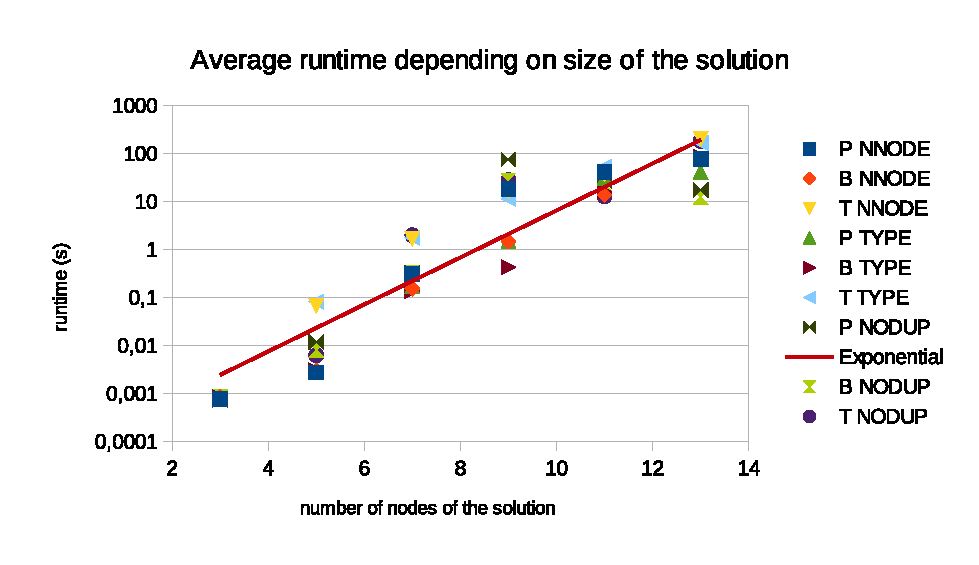
\includegraphics[width=0.95\textwidth]{time_vs_nof_nodes.eps}
    \caption{Average running time of the variants of the synthesis procedure depending on the number of nodes of the solution.}
    \label{fig:runtime_vs_nof_nodes}
\end{figure}
Figure~\ref{fig:runtime_vs_nof_nodes} shows that the average running time for all nine variants of the synthesis procedure depends exponentially on the number of nodes. This goes along with the intuition that a bigger program is more difficult to synthesise.
For example, if we have $n$ possibilities to generate a program consisting of one node, that is \lstinline!?x! where we have $n$ possibilities to instantiate the hole \lstinline!?x!, then we will have $n^2$ possibilities to generate a program with three nodes, that is \lstinline!?$x_1$ ?$x_2$! where we have $n$ possibilities to instantiate the hole.


\TODO{Delete this question or do something with it. We cannot answer it, we do not have enough data.}
More surprisingly, the individual results show that there must be some other factor influencing the runtime. Take, for example, \lstinline?enumFromTo?, \lstinline?stutter? and \lstinline?nth?. All three of them have a solution with exactly $13$ nodes, but their runtimes differ at least by an order of magnitude. What does make \lstinline?nth? generate in less than \SI{1}{s}, \lstinline?stutter? a hundred times slower and \lstinline?enumFromTo? to time out in most of the cases?

In our simple intuitive explanation of the exponential dependency of the synthesis time with the size of the solution we completely ignored the contribution of types to search space pruning.


\subsection{Type of the solution}
polymorphic easier to synthesise because less functions apply. nth vs stutter vs enumFromTo.
discuss together with type of components.

\TODO{why does enumFromTo take so much time even with enumTo as a component}
\TODO{we can actually synthesise enumFromTo without enumTo and we actually did in a very restricted context (only the library components present in the actual solution), but it takes a lot of time.}
\subsection{Number of components}
\subsection{Examples}
\subsection{Blacklist}
\subsection{Templates}
\subsection{Cost functions}
\subsection{Stack vs Queue expansion}

\section{Interesting unexpected solutions}
\TODO{explain the thing with the different solutions\\}
\TODO{discuss interesting solutions, isEven, member\\}
\TODO{polymorphic equality\\}
\section{Automatic black list}\label{Automatic black list}

\section{Comparison to related work}








----------------------------------------
What I want to see in this chapter:
\begin{itemize}
\item runtime highly dependent on the number of components used in the solution \TODO{if you have time, redo the graph relating number of components to runtime in latex}
\item difficult to find examples (small but enough)
Sensible to the choice of examples: for speed (enumTo prod enumTo prod...), examples must be small and there must be only a few of them. But then it is very likely, that another program is generated. It is very tricky to choose the right examples for enumFromTo and for member.
\item blacklist tradeoff: Show advantages of using black lists and explain why we do not see them in the data. (we do see them. Compare plain nof-nodes with blacklist nof-nodes. The benefit is comparable with the introduction of the nof-nodes-simple-types cost function. Which is reasonable, because they both fight against \lstinline?head nil?.)
\item Table of all components (no, this should go to implementation)
\item Table of synthesized programs with synthesis times for the different algorithms (aka giant-table-19 and giant-table-37)
\item Figure of the synthesis times of synthesized programs (nope)
\item Comparison to Feser, to Nadia, to Escher and to Myth (yes, we have their running times for some of the benchmarks. Say that you cannot really compare the numbers because they weren't run on the same machine).
\item Explain why automatic black list generation did not worked out as you wished
\begin{itemize}
\item only identity function (but you could also generate something else)
\item many "useless" programs already ruled out by other programs (but you could incrementally use the blacklist as a blacklist, you know?)
\item (maybe) show it?
\end{itemize}
\item Explain why templates perform so poorly (hm... because they don't do BFS, that is they have to explore every branch to the "end"?)
\item How number of components affects synthesis time
\begin{itemize}
\item In particular, not only the number but also the number of components of the same type. If you have more functions with the same type you will need much more time to find the program you are looking for (more possible successors).
\end{itemize} 
\item Talk about the constants in the cost functions and how they affect the search space.
How cost functions influence the search space (\lstinline!(head (^26 -> ^27 -> Int) (nil (^26 -> ^27 -> Int))) ?2 ?3! has too complicated types appearing in the term, so it will have a higher cost in some of the cost functions. \lstinline!foldnat foldnat foldnat mul (mul 3 3) 3! takes a lot of time to evaluate, it will have a higher cost in no-same-component).
\begin{itemize}
\item Idea behind nof-nodes: smaller programs generalize better to the examples
\item Idea behind nof-nodes-simple-types: programs with smaller types are less "useless" (example with \lstinline?head nil?). Favor the use of input variables. But now a lot of "simple" but difficult to evaluate programs are synthesised, like the \lstinline?enumTo prod enumTo prod?.
\item Idea behind no-same-component: there are components that are usually used only once in a program, like \lstinline?foldr?, \lstinline?foldNat?. Another thing is that we penalize also complicated types of the form \lstinline?List (List (^5 -> List ^4))? that had no additional cost in nof-nodes-simple-types. But now types overweight the number of nodes and simple programs like \lstinline?foldr add zero _0? weight more than programs like \lstinline?add mul sub prod enumTo...?.
\item Idea behind no-same-component-bigger-constants: make all constants bigger so that we can differentiate more between the constants and so that nodes count more than types.
\item Idea behind no-same-component-even-bigger-constants: see above. (well, then you failed. your constants for types are pretty much as big as those for terms...). Why it's bad? See above.
\end{itemize}
\item Stack versus queue expanding $\rightarrow$ mention it in the definitions (argument why stack is better. Intuitively it makes sense to construct a program from top-down or bottom-up, but it does not make any sense to put in some components in the middle. \lstinline!?1 ?2! gets transformed to \lstinline!(?3 ?4) ?2! and then we get programs like \lstinline!(?3 ?4) sum! and \lstinline!(?3 ?4) foldr! for all possible components. The leftmost strategy makes much more sense, because then we put constraint on the type of the next hole to be expanded.
\end{itemize}

\section{Set up}
  \note{Describe the machine and the testing set up, which components were used, what information did you give to the synthesizer, how many examples were given. What else?}
All experiments were run on an Intel quad core 3.2~GHz with 16~GB RAM. Since the code is sequential, the performance could not benefit from the number of cores.

We refer to Table~\ref{giant_table_19} and Table~\ref{giant_table_37} for the experimental results. All performance numbers are averages from 1 to 3 different executions all sharing the same specification. The goal type and the given examples do not change between different executions. In Table~\ref{giant_table_37} all benchmarks share the same set of components.

\section{Specification size}

\section{Solution size}
  
\section{Cost functions}
  \note{Compare the different cost functions with each other, explain why are they good for some programs and bad for other. Table.}

\section{Black lists}

In the presence of "useless" functions with a high branching factor like \lstinline?flip?, \lstinline?const? or \lstinline?uncurry? black list pruning is a must. But it can also be useful in other cases as well. The important thing is to find a reasonable trade off between the length of the black list (don't forget that every subterm of every open program is matched against every item of the black list) and the degree of pruning. A longer black list prunes more of the search space, but the synthesis procedure also takes longer.

  \subsection{Benefits of black lists}
  \note{Table of your super manual black list. Figure that for each cost function compares time with and without black list. Trivial words about pruning search space and useless branches.}
  \subsection{Shortcomes of automatically generated black lists}
  \note{Maybe really bring the automatically generated table. Point at the repetitions. Say that automatically generated I/O-examples are bad and we need a lot of them. Say that you tried only identity pruning, but one could also try to generate, say, the empty list or whatever.}

\section{Templates}
  \note{Short section explaining that the templates you generate are not the templates you expect and why}
I found one example, where templates help! For \lstinline?dropmax? I had a run out of memory exception with plain enumeration and I could synthesise it in 7 seconds with templates!
(Ok, I modified templates to put in only really higher-order components and close every hole, no matter the type).

It is very important to choose the examples well, because many generated programs are bad and will take forever to evaluate. And as we evaluate each closed program on the examples... We should really try to keep them small and simple.
For example, I had a problem when I tried to generate \lstinline?dropmax? using the example \lstinline?[1,4,3]?, because one of the generated programs was \lstinline?enumTo (prod (enumTo (prod _0)))?. It tried to construct a list with 479001600 elements and ran out of memory.
At the same time, they should give enough information, otherwise a simpler program will be generated that, although it satisfies all given I/O-examples, it not what the user had in mind when writing the specification.

%%% Local Variables:
%%% mode: latex
%%% TeX-master: "thesis"
%%% End:

\chapter{Conclusions} \label{ch:conclusions}

\section{Conclusions}

Type-driven synthesis of functional programs from input-output examples   strives to automatically generate well-typed programs that satisfy the given input-output examples and generalise well to unseen input-output pairs. When solving similar tasks, human programmers rely on well-known computational patterns.

%\TODO{Do we need the example at all?\\}
%Consider, for example, a human is given the task to write \lstinline!replicate!, the function that takes an integer \lstinline!n! and an element \lstinline!x! and returns the list \lstinline![x, x, $\ldots$, x]! of \lstinline!n! copies of \lstinline!x!. The human would probably resort to recursion over integers. That is, depending on the value of \lstinline!n!, she would either call \lstinline!replicate (n-1) x! and prepend the result with another \lstinline!x! or, if \lstinline!n! is $0$, return the empty list:
%\begin{lstlisting}[style=plain]
%replicate 0 x = []
%replicate n x = x:(replicate (n-1) x)
%\end{lstlisting}
%This computational pattern is expressed by \lstinline!foldNat!, the higher-order component that folds an integer using a given function. That is, the above program is equivalent to:
%\begin{lstlisting}[style=plain]
%replicate n x = foldNat (x:) [] n
%\end{lstlisting}

The main goal of the thesis was to study how well first- and higher-order components can guide and speed up the synthesis process.

In order to achieve this goal, we implemented in OCaml a prototype of a simple synthesis procedure based on program enumeration. Extensive evaluation of the prototype on benchmarks showed that it can compete with related state-of-the-art tools. We believe therefore that synthesis from library components is a promising direction and needs to be explored further.

The prototype implements a synthesis procedure based on best-first enumeration of partial programs. We experimented with different cost functions and with different strategies to expand a partial program.

During experimentation we faced different classes of programs that hinder the synthesis process.

First of all, we discovered that the search space abounds of closed programs that represent a challenge for our evaluator, even on examples as small as \lstinline![2,2,3]! and \lstinline!3!. This was our main motivation to reduce the size and the number of input-output examples.

Next, we noticed that every hole can be filled in with \lstinline!head [?X] (nil [?X])!, where \lstinline!?X! has to be instantiated with the type of the hole to expand. Many partial programs containing this pattern were enumerated just to be ruled out as soon as all holes were filled in and the closed programs were evaluated. To prune whole branches that will surely not lead to a solution, we introduced a black list containing the undesired patterns. As a next step, we used the synthesiser to generate such a black list automatically.

A related problem are partial programs that can be ruled out based on the semantics of the library component and the expected behaviour of the target program. For example, when trying to synthesise \lstinline!enumFromTo!, no human programmer would insist on taking \lstinline!enumTo! as the first component. The partial program
\begin{lstlisting}[style=plain]
enumFromTo m n = enumTo ?x
\end{lstlisting}
will not lead to the solution, because every list returned by \lstinline!enumTo!, no matter the argument, starts with $1$, whereas the list returned by \lstinline!enumFromTo! should start with \lstinline!m!, which is not necessarily $1$. Our synthesis procedure, on the contrary, treats this partial program and its successors as very promising candidates.\\
This motivated us to try a slightly different synthesis procedure: the one that fixes the higher-order components first (generating a \emph{template}) and then fills in the remaining holes with input variables and first-order components.

We also explored some rudimentary ways of user-synthesiser interaction in order to help the synthesiser to avoid those three classes of undesired programs.

The simplest way to help the synthesiser is to restrict the library to the components needed for the synthesis task at hand. For example, the user might expect that \lstinline!enumFromTo! can be synthesised by putting together \lstinline!enumTo!, \lstinline!map!, \lstinline!add!, \lstinline!sub! and the integer and lists constructors. However, in our experience it is easy to miss some of the components.

Another way to help the synthesiser generating helper functions first and adding them to the library before the synthesis of the desired program. For example, to speed up the synthesis of \lstinline!enumFromTo!, we first generated \lstinline!enumTo! from the components we had. This increases the size of the library, but reduces the size of the generated solution.

The last way to help the synthesiser we tried is to specify a starting template. For example, the user might have the intuition that \lstinline!enumFromTo! can be synthesised by adding some integer to each element of a list of consecutive numbers. She can encode this intuition into the template:
\begin{lstlisting}[style=plain]
enumFromTo m n = map [Int] [Int] (add ?i) (enumTo ?j)
\end{lstlisting}
and get the desired implementation:
\begin{lstlisting}[style=plain]
enumFromTo m n = map [Int] [Int] (add (sub m (succ zero))) (enumTo (succ (sub n m)))
\end{lstlisting}
However, user-input is usually not needed to synthesise the benchmarks in less than a minute, \lstinline!enumFromTo! being the only exception.

Empirical evaluation showed that reducing the size of the examples and blacklisting undesired patterns improves, as expected, the performance. On the other hand, against expectations, the introduction of templates leads to a significant slowdown. We believe, however, that this is due to our implementation and should be investigated further.
  
\section{Future Work}

As anticipated in the previous section, the information about well-known computational patterns encoded as library components can be successfully reused in program synthesis, and this promising direction needs further exploration. In this section we list some possibilities for future work that follow from the limitations of our system.

Pruning based on black lists helps to reduce synthesis time. However, manually compiled black lists are inconvenient when users are allowed to add their own components to the library. Automatically synthesising a black list from the components in the given library would leverage this inconvenience. In Section~\ref{Black list generation} we discussed the limitations of an automatically generated black list. In particular, since the automatically generated patterns are closed, they do not generalise. For example, instead of the following patterns expressing that folding over an empty list is an unnecessarily long synonym for the initial value
\begin{lstlisting}[style=plain]
foldr append _ nil
foldr const _ nil
foldr drop _ nil
\end{lstlisting}
we would like to have in our black list the following more general pattern:
\begin{lstlisting}[style=plain]
foldr _ _ nil
\end{lstlisting}
In general, a good automatically generated black list should contain only the shortest most general patterns corresponding to the identity function, to the constructors and to other simple terms.
We believe that generalisation of patterns could be, at least partially, addressed by partial evaluation of programs with holes.

A very interesting question that our thesis does not answer is whether fixing the higher-order functions first in form of templates helps to guide and speed up synthesis. As discussed in Section~\ref{Eval. Templates}, the successor rules currently used in our prototype implementation generate a lot of undesirable templates such as:
\begin{lstlisting}[style=plain]
?x (foldr [?X] [?Y])
?x (map [?$X_1$] [?$Y_1$]) (foldr [?$X_2$] [?$Y_2$])
\end{lstlisting}
Rewriting the successor rules or pruning templates according to some heuristic could shed light on the practical impact of this approach on synthesis time. In particular, we believe that limiting the size of the programs being synthesised instead of the depth of the first-order search could be a first step towards a more efficient implementation. Reason for it is that undesirable templates tend to have very few successors in the first-order search. As a result, partial programs being explored are typically quickly growing applications of holes.

In the previous section we additionally saw three ways the user can help the synthesiser. Another clue the user could provide, along with the input-output examples, is some intermediate value that can be produced from the given input and is used in the computation of the output.
For example, consider we want to synthesise \lstinline!enumFromTo m n!. The list of consecutive integers from $m$ to $n$ can be computed from the list of consecutive integers from $1$ to $n-m+1$ by adding $m-1$ to each element. That is, the user could specify the synthesis task providing following \emph{augmented examples}, the rightmost list being the expected output:
\begin{lstlisting}[style=plain]
enumFromTo 1 2 $\rightsquigarrow$ [1,2] $\rightsquigarrow$ [1,2]
enumFromTo 3 4 $\rightsquigarrow$ [1,2] $\rightsquigarrow$ [3,4]
enumFromTo 2 5 $\rightsquigarrow$ [1,2,3] $\rightsquigarrow$ [2,4,5]
\end{lstlisting}
The synthesiser would come up with the solution (where we substitute fully applied \lstinline!add! and \lstinline!sub! with the corresponding infix operators and \lstinline!succ zero! with $1$):
\begin{lstlisting}[style=plain]
enumFromTo m n = map [Int] [Int] (add (m-1)) (enumTo (n-m+1))
\end{lstlisting}
The open question is how to use the augmented examples to restrict the search space and suggest the relevant library components to the synthesiser. 
Moreover, the user-synthesiser interaction can be brought to a new level by permitting the synthesiser to explicitly ask the user for help. For example, when coming up with intermediate values, the synthesiser could ask whether they are relevant to the current synthesis task.



%%% Local Variables:
%%% mode: latex
%%% TeX-master: "thesis"
%%% End:


%%\chapter{Baseline} \label{baseline}

\section{Syntax}
\note{
it's the description of the syntax of the programs in the search space as well as how to derive programs from programs. 
}

\note{Rewrite this without mixing syntax with semantics and with the baseline algorithm}
In the context $\Gamma$ we store the bindings from library components and input variables to their types.

In the context $\Delta$ we store the bindings from active and inactive holes to their types.

Terms are applications of library components or input variables (denoted by $x$ in the grammar), values (denoted by $v$) and holes ($?x$ and $?\underline{v}$).

We distinguish between active holes $?x$, that can be substituted with other programs, from inactive holes $?\underline{v}$, that can only be replaced with values. To determine the exact value, a heuristic using a mix of symbolic execution and brute force is applied later. Every active hole having a value type (denoted by $V$ in the grammar) can be turned into an inactive hole.

Programs without active holes are considered \emph{closed}. Those are the programs in which we plug in the input and execute as far as possible to see whether it agrees with the expected output.

Values are integer constants (denoted by $n$ for brevity), lists of values and tuples of values. \note{Does it make sense to have a special treatment for list values and tuples? Wouldn't it be better to use library components to construct them?}

We use a standard type system featuring functional and universal types, as well as integers, lists and tuples. We distinguish between two kinds of type variables: $?X$ are the type variables that can be instantiated with other types when it comes to unification, $X$ are the type variables that are already fixed by the goal type and have to remain like that. Universal types are assumed to be used like in Haskell only as outer wrapping of the types of library components and the goal type specified by the user.

\TODO{Find a way to format t t as t t and not a tt, same for VV and TT}
\TODO{Find a way to format it vertically and adding comments to each line. For example, write "inactive hole" on the right of $?\underline{v}$.}
\note{Maybe it's better to write $\Gamma$ and $\Delta$ as sets and not as grammars, as you are using them as sets. If you leave it like this, $\Delta \setminus \{?x : T\}$ would be undefined.}
\begin{plstx}
(library components): \Gamma ::= \emptyset | \Gamma \cup x : T \\
(holes): \Delta ::= \emptyset | \Delta \cup ?x : T | \Delta \cup ?\underline{v} : T \\
(terms): t ::= v | ?\underline{v} | ?x | x | t t \\
(values): v ::= n | v : v | [] | (v,v) \\ 
(types): T ::= \text{Int} | \text{List } T | \text{Tuple } T T | T \rightarrow T | \forall X. T | X | ?X \\
(value types): V ::= \text{Int} | \text{List } V | \text{Tuple } V V \\
\end{plstx}

\note{It may appropriate to move this to the next section}
We assume that the goal program is normalized in the following sense. If the goal type specified by the user is a universal type, then we substitute each universally quantified type variable with a fresh fixed type variable $X$. If the goal type is a function type, then we abstract the type as much as possible and add input variables to the context $\Gamma$.
For example, if the user specifies the goal program as
\begin{lstlisting}[mathescape]
length :: $\forall X$. List $X$ -> Int
length [1,2,3] == 3
length [2,2,2] == 3
length [] == 0
length [5] == 1
\end{lstlisting}
then we start our search from the partial program $\Gamma \cup \{xs : \texttt{List } X \} \vdash ?x :: \texttt{Int}$ where $\Gamma$ already contains all bindings from library components to their types. Note that it must be possible to instantiate the type variable $X$ with every possible type, therefore we do not have the right to prefer one instantiation over another and must treat $X$ as an uninterpreted type.

\TODO{Add the rules of the typing judgement}
The typing judgement is standard. To define the search graph we are going to explore in order to find the goal program, we also need the \emph{derive} judgement, which says between which nodes of the graph (programs of the form $\Gamma, \Delta \vdash t :: T$) there is an edge.
To express the rules in a more compact form, we introduce \emph{evaluation contexts}. An context is an expression with exactly one syntactic hole $[]$ in which we can plug in any term. For example, if we have the context $\mathcal{E}$ we can place the term $t$ into its hole and denote this new term by $\mathcal{E}[t]$.

\TODO{Make a figure of all rules}
We can turn an active hole into an inactive hole if the active hole has a value type.
\note{do we need a premise? Wouldn't it be enough to write ?x :: V below the line?}
%D-VarVal, if we can turn an active hole into an inactive hole
\begin{prooftree}
\AxiomC{$\Gamma, \Delta \vdash ?x :: V$}
	\RightLabel{D-VarVal}
	\UnaryInfC{$\Gamma, \Delta \vdash ?x :: T \Mapsto \Gamma, \Delta \setminus \{?x : T\} \cup \{?\underline{v} : V\} \vdash ?\underline{v} :: V$}
\end{prooftree}

An active hole $?x$ can be turned into a library component or an input variable $x$ from the context $\Gamma$. The procedure fresh($T$) transforms universally quantified type variables into fresh type variables $?X$ not used in $\Delta$.
The notation $\sigma(\Delta)$ denotes the application of the substitution $\sigma$ to all types contained in the context $\Delta$.
%D-VarComp, an active hole can be turned into a library component or an input variable
\begin{prooftree}
\AxiomC{$x : T_x \in \Gamma$}
\AxiomC{$\sigma$ unifies $T$ with fresh($T_x$)}
	\RightLabel{D-VarLib}
	\BinaryInfC{$\Gamma, \Delta \vdash ?x :: T \Mapsto \Gamma, \sigma(\Delta \setminus \{?x : T\}) \vdash x :: \sigma(T) $}
\end{prooftree}

An active hole can also be turned into a function application of two new active holes.
%D-VarApp, we can turn one hole into two holes :)
\begin{prooftree}
\AxiomC{$?X$ is a fresh type variable}
	\RightLabel{D-VarApp}
	\UnaryInfC{$\Gamma, \Delta \vdash ?x :: T \Mapsto \Gamma, \Delta \setminus \{?x:T\} \cup \{?x_1 : ?X \rightarrow T, ?x_2 : ?X\} \vdash ?x_1$ $?x_2 ::T$}
\end{prooftree}

In all other cases we just choose an active hole and expand it according to the three rules above.
%D-App, for all other cases
\begin{prooftree}
\AxiomC{$\Gamma, \Delta \vdash ?x :: T_1 \Mapsto \Gamma, \Delta' \vdash t_1' :: T_1'$}
	\RightLabel{D-App}
	\UnaryInfC{$\Gamma, \Delta \vdash t[?x] :: T \Mapsto \Gamma, \Delta' \vdash t[t_1] :: T[T_1/T_1']$}
\end{prooftree}

\section{Baseline Algorithm}
\note{
The breadth (or best) first search of the search graph, nothing fancy. 
}

The baseline algorithm is a simple best first search implemented using a priority queue. One possibility is to order the enqueued elements according to the number of library components and active holes.

The root node has the form $\Gamma, \{?x:T\} \vdash ?x :: T$ where $T$ is neither functional nor universal type and $\Gamma$ contains the input variables along with the library components.
The successors of a node are the nodes reachable in one step of the derive judgement. That is, $\Gamma, \Delta' \vdash t' :: T'$ is a successor of $\Gamma, \Delta \vdash t :: T$ if it holds $\Gamma, \Delta \vdash t :: T \Mapsto \Gamma, \Delta' \vdash t' :: T'$.

We don't need to explore nodes that are equivalent up to alpha conversion to already visited nodes.

A term is considered \emph{closed} if it does not contain active holes. Closed terms are tested on the input-output examples. Programs with inactive holes are symbolically executed on the input-output examples and, if possible, the concrete value of the inactive hole is determined. Otherwise we try to solve it by brute force with a small timeout.
\note{Does it make sense in terms of performance? Usually the values we need are really simple like \lstinline?[], 0, 1?. Wouldn't it be more efficient to try some simple values first?}

The input-output examples are given as a vector of inputs \lstinline?I? and the vector of corresponding expected outputs \lstinline?O?.

\TODO{Typeset in a nicer way, for example with a vertical line instead of all those 'end' and nicer keyword formatting.}
\begin{lstlisting}[mathescape]
BFS(root, I, O)
	queue $\leftarrow$ {root}
	visited $\leftarrow$ {}
	while($\text{timeout not reached}$)
		current $\leftarrow$ queue.dequeue
		if (current.closed)
			if (current.test(I) == O)
				return current
			end
		else
			for (s in current.successors)
				if (!visited.alphacontains(s))
					queue $\leftarrow$ queue.push(s)
				end
			end
		end
	end
end
\end{lstlisting}



%%% Local Variables:
%%% mode: latex
%%% TeX-master: "thesis"
%%% End:

%%\chapter{Benchmarks} \label{benchmarks}

\note{
Some programs over numbers, some over lists, some over lists of lists and some over trees (What kind of trees?).
For every program, try to get a sample implementation. \\
Types needed: \lstinline?Int, [a], Tree a? \\
Basic components needed:
arithmetic (\lstinline?+, -, *, /?), 
relation (\lstinline?<, <=, ==, /=, >=, >?),
\note{(maybe we do not need relations)}
}

\begin{enumerate}
	\item max of two numbers\\
	(hopefully) the easiest program \\
	\begin{lstlisting}
max :: Int -> Int -> Int
max 0 0 == 0
max 1 0 == 1
max 0 1 == 1
max x y = if x > y then x else y
	\end{lstlisting}
	\note{We don't care about conditionals, we cannot synthesize this.}\\
	This is the only function that requires a conditional branch.
%
	\item square a number
	\begin{lstlisting}
square :: Int -> Int -> Int
square 0 == 0
square 1 == 1
square 2 == 4
square 3 == 9
square x = x * x
	\end{lstlisting}
	That is, basic arithmetic operations like \lstinline!+ - * /! should be provided
%
	\item tetrahedral numbers \\
	\begin{lstlisting}
tetrahedral :: Int -> Int
tetrahedral 1 == 1
tetrahedral 2 == 4
tetrahedral 3 == 10
	\end{lstlisting}
	closed form solution
	\begin{lstlisting}
tetrahedral n = n * (n+1) * (n+2) / 6
	\end{lstlisting}
	iterative solution
	\begin{lstlisting}
tetrahedral n = scanl1 (+) (scanl1 (+) [0..]) !! n
	\end{lstlisting}
	Another iterative solution (without infinite lists)
	\begin{lstlisting}
tetrahedral n = foldl1 (+) (scanl1 (+) (enumFromTo 1 n))
	\end{lstlisting}
	Components needed: \lstinline?scanl1, !!? \\
	Interestingly the iterative version is much faster than the closed form solution
%
	\item prime test \\
	I think this is too difficult
	\begin{lstlisting}
prime :: Int -> Int
prime 1 == 0
prime 2 == 1
prime 3 == 1
prime 4 == 0
prime 25 == 0
prime 29 == 1
prime n = minimum (1 : (map (mod n) (enumFromTo 2 (subtract 1 n))))
	\end{lstlisting}
	Components needed: \lstinline?map, mod, minimum, enumFromTo, subtract?
%
	\item average
	\begin{lstlisting}
average :: [Int] -> Int
average [1] == 1
average [1,3] == 2
average [1,2,3,6] == 6
average xs = (sum xs) `div` (length xs)
	\end{lstlisting}
%
	\item movingAverage (forward)
	\begin{lstlisting}
movingAverage :: Int -> [Int] -> [Int]
movingAverage 1 [1,2,3] == [1,2,3]
movingAverage 2 [1,2,3] == [2,2,3]
movingAverage 3 [3,2,4,1,5,2] == [3,2,3,2,3,2]
movingAverage n xs = map (average . take n) (init $ tails xs)
	\end{lstlisting}
	Components needed: \lstinline?tails? from \lstinline?Data.List? and  \lstinline?average? (one of the benchmarks), as well as \lstinline?map, take? and \lstinline?init? from \lstinline?Prelude?.
%
	\item movingSum (backward)
	\begin{lstlisting}
movingSum :: Int -> [Int] -> [Int]
movingSum 1 [1,2,3] == [1,2,3]
movingSum 2 [1,2,3] == [1,3,5]
movingSum 3 [4,8,6,-1,-2,-3,-1,3,4,5] == [4,12,18,13,3,-6,-6,-1,6,12]
movingSum n xs = scanl1 (+) (zipWith (-) xs (replicate n 0 ++ xs))
	\end{lstlisting}
%
	\item waterflow problem \\
	Given an array of "wall" heights, determine the volume of the puddles that can form if it rains.
	\begin{lstlisting}
water :: [Int] -> Int
water [1,2,3] == 0
water [5,2,5] == 3
water [2,3,1,6,1] == 2
water h = sum $ 
      zipWith (-) 
        (zipWith min (scanl1 max h) (scanr1 max h))
        h
	\end{lstlisting}
%
	\item horner schema to evaluate polynomials
	\begin{lstlisting}
horner :: [Int] -> Int -> Int
horner [1,2,3] 1 == 6
horner [1,2,3] 2 == 11
horner [4,3,2] 3 == 47
horner p x = foldl1 ((+) . (x *)) p
	\end{lstlisting}
	Problem: we do not generate lambda's. Do we generate functions like \lstinline?(x *)??
%
	\item sum-under, sum all integers up to the argument
	\begin{lstlisting}
sum_under :: Int -> Int
sum_under 0 == 0
sum_under 1 == 1
sum_under 2 == 3
sum_under 3 == 6
sum_under 4 == 10
sum_under n = sum [1..n]
	\end{lstlisting}
	Components needed: \lstinline?sum, enumFromTo?
%
	\item factorial \\
	\begin{lstlisting}
factorial :: Int -> Int
factorial 0 == 0
factorial 1 == 1
factorial 3 == 6
factorial 5 == 120
factorial n = product [1..n]
	\end{lstlisting}
	interesting for intermediate states
%
	\item maximum of a list\\
	I don't know (yet) how to specify a "global property" like greater or smaller than all other elements in a list in \textsc{Synquid}. Moreover, it seems a difficult property to extract from input-output examples.
	\begin{lstlisting}
maximum :: [Int] -> Int
maximum [1,3,2] == 3
maximum [4,2,1] == 4
maximum [1,3,5] == 5
maximum xs = foldr max (head xs) xs
	\end{lstlisting}
	Or just use the \lstinline?maximum? function from \lstinline?Prelude?, if it is given as a component
%
	\item append two lists\\
	The specification given by Nadia does not synthesize the usual append function. Maybe it's better to let her know...\\
	Although it's possible to synthesize append in \textsc{Synquid}.
	\begin{lstlisting}
append :: [a] -> [a] -> [a]
append [1,2,3] [4,5,6] == [1,2,3,4,5,6]
append [1,2] [6,2,3] == [1,2,6,2,3]
append xs ys = foldr (:) ys xs
	\end{lstlisting}
	Or use \lstinline?++? from \lstinline?Prelude?, if we decide to provide it for this example too.
%
	\item length of a list \\
	Can be also interesting for intermediate states
	\begin{lstlisting}
length :: [a] -> Int
length [1,2,3] == 3
length [2,2,2] == 3
length [] == 0
length [5] == 1
length xs = sum $ map (const 1) xs
	\end{lstlisting}
%
	\item list reversal
	\begin{lstlisting}
reverse :: [a] -> [a]
reverse [1,2,3] == [3,2,1]
reverse [5,2,3] == [3,2,5]
reverse [6,2,3,1] == [1,3,2,6]
reverse xs = foldl (flip (:)) [] xs
	\end{lstlisting}
%
	\item bagsum: \lstinline![far,bar,gar,bar,bar,far] -> [(bar,3),(far,2),(gar,1)]!\\
	Seems difficult and maybe intermediate states can be helpful. Should I take \lstinline?Int? instead of \lstinline?a?? I mean, \lstinline?a? should belong to the typeclass \lstinline?Ord?, otherwise we cannot yield a sorted output list. And we do not have any other base types anyway. But actually lists of integers are also ordable. Hence also lists of lists of integers and lists of lists of lists of integers and so on.
	\begin{lstlisting}
bagsum :: [a] -> [(a, Int)]
bagsum [1,1,1] == [(1,3)]
bagsum [4,4,2,1,2,1] == [(1,2),(2,2),(4,2)]
bagsum [3,2,1,3,2,3] == [(1,1),(2,2),(3,3)]
bagsum xs = map (head &&& length) (group (sort xs))
	\end{lstlisting}
	Components needed: \lstinline?&&&? from \lstinline?Control.Arrow?. And we also need \lstinline?Tuples? for this one.
%
	\item map \\
	Isn't it a higher order function? I thought we synthesize only first order functions.\\
	How can we provide examples? I mean, we have to write functions as well.\\
	\begin{lstlisting}
map :: (a -> b) -> [a] -> [b]
map f xs = foldr ((:) . f) [] xs
	\end{lstlisting}
%
	\item zipWith \\
	it's a higher order function as well. We need Tuples.\\
	How do we provide the examples?
	\begin{lstlisting}
zipWith :: (a -> b -> c) -> [a] -> [b] -> [c]
zipWith f xs ys = map (uncurry f) (zip xs ys)
	\end{lstlisting}
	Components needed: \lstinline?map, uncurry, zip?.
%
	\item list drop
	\begin{lstlisting}
drop :: Int -> [a] -> [a]
drop 0 [1,2,3] == [1,2,3]
drop 1 [1,2,3] == [2,3]
drop 5 [5,4,2,5] == []
drop 3 [4,2,3,1] == [1]
drop n xs = snd (splitAt n xs)
	\end{lstlisting}
%
	\item droplast, drop the last element of a list
	\begin{lstlisting}
droplast :: [a] -> [a]
droplast [] == []
droplast [1] == []
droplast [1,2,3] == [1,2]
droplast [3,2,1]== [3,2]
droplst = init
droplast' xs = map fst (zip xs (enumFromTo 1 (subtract 1 (length xs))))
droplast'' xs = take (subtract 1 (length xs)) xs
	\end{lstlisting}
%
	\item dropmax, drop the greatest element of a list\\
	$\lambda^2$ takes much more time to synthesize droplast than dropmax. Why?
	\begin{lstlisting}
dropmax :: [Int] -> [Int]
dropmax [1,2] == [1]
dropmax [2,1] == [1]
dropmax [1,2,3] == [1,2]
dropmax [3,2,1] == [2,1]
dropmax [2,3,1] == [2,1]
dropmax xs = filter (/= (maximum xs)) xs
	\end{lstlisting}
%
	\item dedup, remove duplicates from a list \\
	$\lambda^2$ requires more time\\
	\TODO{Find a non-recursive implementation that preserves the order of the elements} Either implement it with \lstinline?groupBy? or say you cannot implement it. Say it's not possible to get the usual semantics of deleting all but the first occurrence of some program.
%
	\item sort by length (on lists of lists)
	\begin{lstlisting}
sortByLength :: [[a]] -> [[a]]
sortByLength [[1,2],[1,2,3],[1]] == [[1],[1,2],[1,2,3]]
sortByLength = sortBy (curry ((uncurry compare) . (length *** length)))
	\end{lstlisting}
	\TODO{Is there a shorter implementation?} What's wrong with this one? \\
	Components needed: \lstinline?(***)? from \lstinline?Control.Arrow?
%
	\item dropmins \\
	$\lambda^2$ required more time to synthesize it
	\begin{lstlisting}
dropmins :: [[Int]] -> [[Int]]
dropmins [[1,2,3],[2,3,1],[2,3],[1]] == [[2,3],[2,3],[3],[]]
dropmins = map dropmin
	\end{lstlisting}
	\TODO{Is there an implementation without the auxiliary function \lstinline?dropmin? and without lambda expressions?} Yes, there is one, but you don't want to see it. With \lstinline?ap? and \lstinline?join?.
%
	\item lasts, last element of every list \\
	another program on nested lists
	\begin{lstlisting}
lasts :: [[a]] -> [a]
lasts [[1,2,3],[3,2],[4,2,4,1],[2]] == [3,2,1,2]
lasts = map last
	\end{lstlisting}
%
	\item member of the tree\\
	Something with trees. Membership seems a difficult thing to learn from input-output examples.
%
	\item count leaves it a tree
%
	\item nodes at level
	The standard Haskell tree is a rose tree. Defined in \lstinline?Data.Tree?.
	
\note{Nadia has more complicated examples with Red-Black-Trees, AVL-trees and different sorting algorithms}
\end{enumerate}




%%% Local Variables:
%%% mode: latex
%%% TeX-master: "thesis"
%%% End:


\appendix

\chapter{Dummy Appendix}

You can defer lengthy calculations that would otherwise only interrupt
the flow of your thesis to an appendix.


\backmatter

\bibliographystyle{plain}
\bibliography{refs}

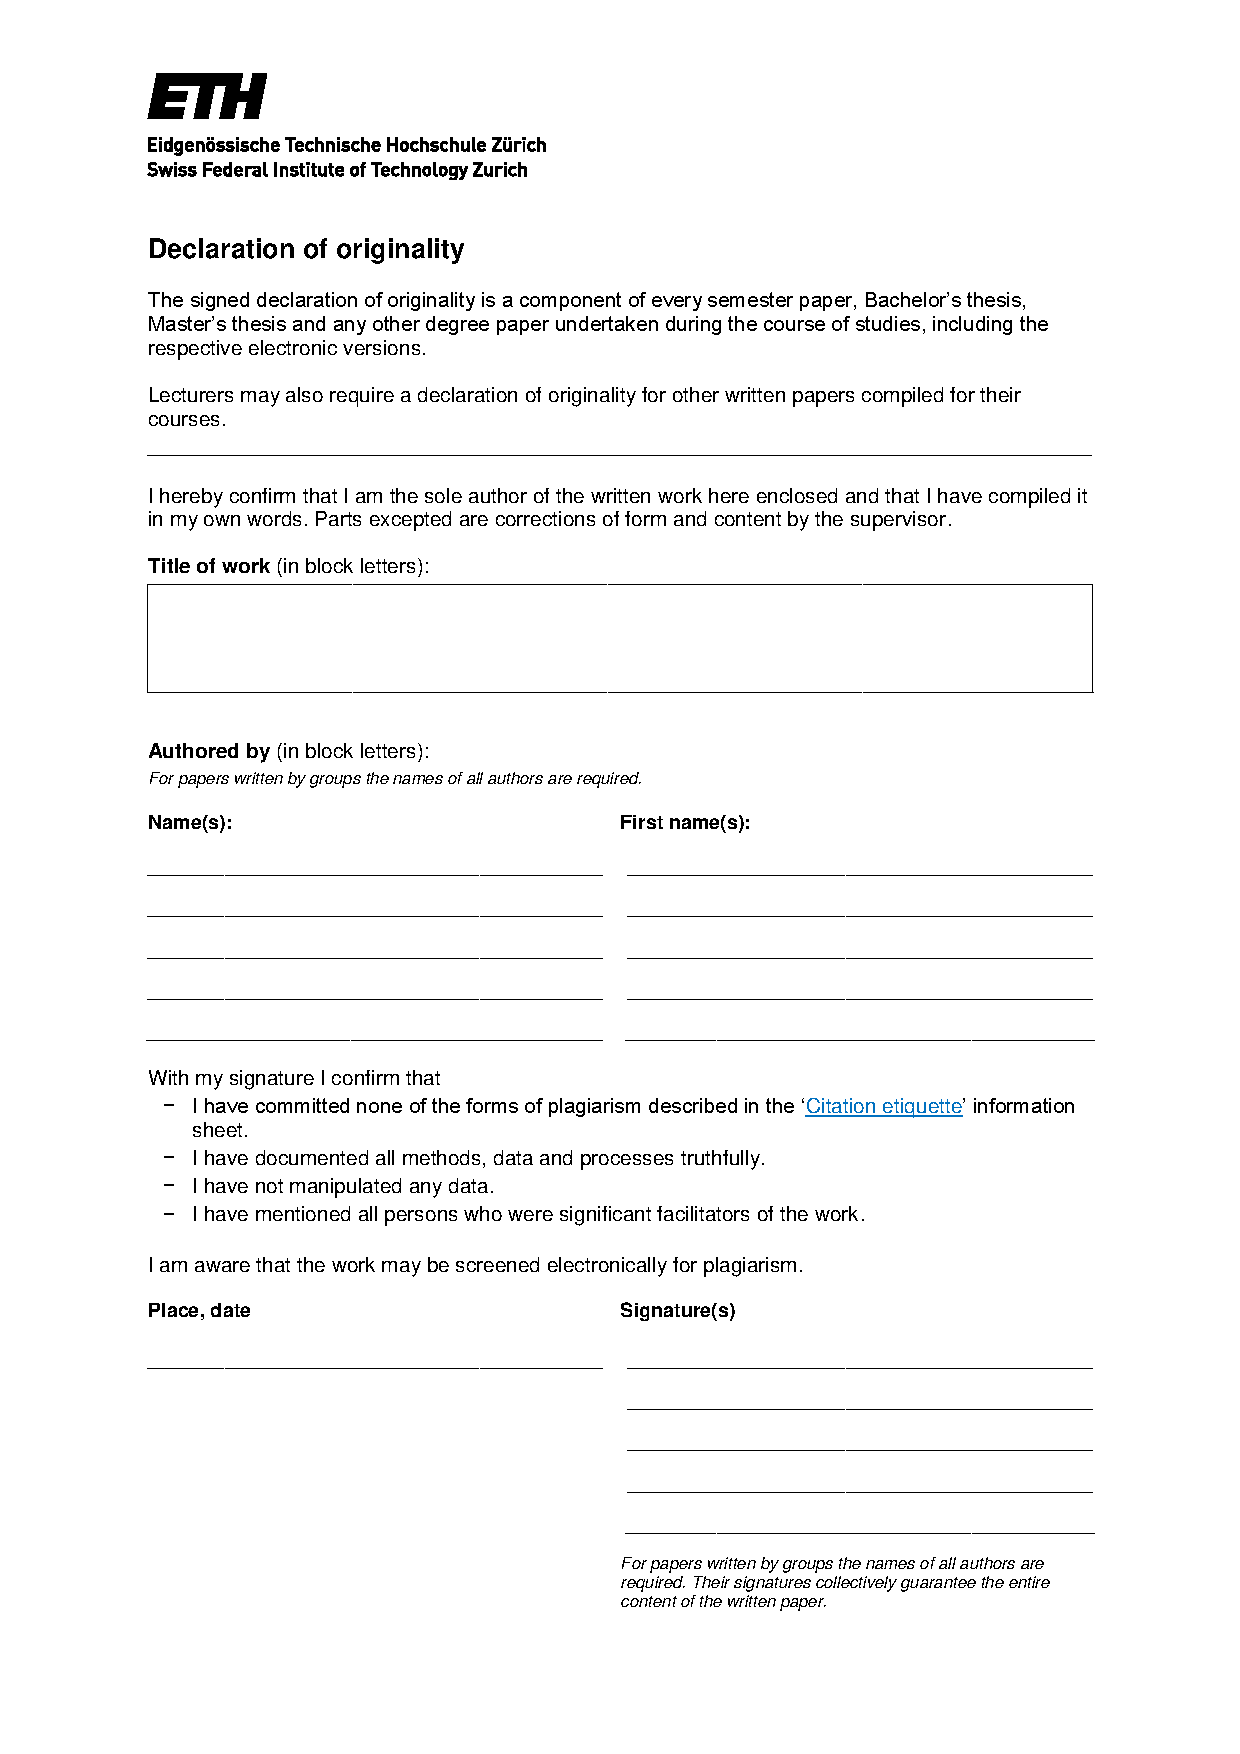
\includepdf[pages={-}]{declaration-originality.pdf}

\end{document}
